\PassOptionsToPackage{unicode=true}{hyperref} % options for packages loaded elsewhere
\PassOptionsToPackage{hyphens}{url}
%
\documentclass[
]{article}
\usepackage{lmodern}
\usepackage{amssymb,amsmath}
\usepackage{ifxetex,ifluatex}
\ifnum 0\ifxetex 1\fi\ifluatex 1\fi=0 % if pdftex
  \usepackage[T1]{fontenc}
  \usepackage[utf8]{inputenc}
  \usepackage{textcomp} % provides euro and other symbols
\else % if luatex or xelatex
  \usepackage{unicode-math}
  \defaultfontfeatures{Scale=MatchLowercase}
  \defaultfontfeatures[\rmfamily]{Ligatures=TeX,Scale=1}
  \setmainfont[]{Lato}
\fi
% use upquote if available, for straight quotes in verbatim environments
\IfFileExists{upquote.sty}{\usepackage{upquote}}{}
\IfFileExists{microtype.sty}{% use microtype if available
  \usepackage[]{microtype}
  \UseMicrotypeSet[protrusion]{basicmath} % disable protrusion for tt fonts
}{}
\makeatletter
\@ifundefined{KOMAClassName}{% if non-KOMA class
  \IfFileExists{parskip.sty}{%
    \usepackage{parskip}
  }{% else
    \setlength{\parindent}{0pt}
    \setlength{\parskip}{6pt plus 2pt minus 1pt}}
}{% if KOMA class
  \KOMAoptions{parskip=half}}
\makeatother
\usepackage{xcolor}
\IfFileExists{xurl.sty}{\usepackage{xurl}}{} % add URL line breaks if available
\IfFileExists{bookmark.sty}{\usepackage{bookmark}}{\usepackage{hyperref}}
\hypersetup{
  pdftitle={Statistical analysis},
  pdfborder={0 0 0},
  breaklinks=true}
\urlstyle{same}  % don't use monospace font for urls
\usepackage[margin=1in]{geometry}
\usepackage{color}
\usepackage{fancyvrb}
\newcommand{\VerbBar}{|}
\newcommand{\VERB}{\Verb[commandchars=\\\{\}]}
\DefineVerbatimEnvironment{Highlighting}{Verbatim}{commandchars=\\\{\}}
% Add ',fontsize=\small' for more characters per line
\usepackage{framed}
\definecolor{shadecolor}{RGB}{248,248,248}
\newenvironment{Shaded}{\begin{snugshade}}{\end{snugshade}}
\newcommand{\AlertTok}[1]{\textcolor[rgb]{0.94,0.16,0.16}{#1}}
\newcommand{\AnnotationTok}[1]{\textcolor[rgb]{0.56,0.35,0.01}{\textbf{\textit{#1}}}}
\newcommand{\AttributeTok}[1]{\textcolor[rgb]{0.77,0.63,0.00}{#1}}
\newcommand{\BaseNTok}[1]{\textcolor[rgb]{0.00,0.00,0.81}{#1}}
\newcommand{\BuiltInTok}[1]{#1}
\newcommand{\CharTok}[1]{\textcolor[rgb]{0.31,0.60,0.02}{#1}}
\newcommand{\CommentTok}[1]{\textcolor[rgb]{0.56,0.35,0.01}{\textit{#1}}}
\newcommand{\CommentVarTok}[1]{\textcolor[rgb]{0.56,0.35,0.01}{\textbf{\textit{#1}}}}
\newcommand{\ConstantTok}[1]{\textcolor[rgb]{0.00,0.00,0.00}{#1}}
\newcommand{\ControlFlowTok}[1]{\textcolor[rgb]{0.13,0.29,0.53}{\textbf{#1}}}
\newcommand{\DataTypeTok}[1]{\textcolor[rgb]{0.13,0.29,0.53}{#1}}
\newcommand{\DecValTok}[1]{\textcolor[rgb]{0.00,0.00,0.81}{#1}}
\newcommand{\DocumentationTok}[1]{\textcolor[rgb]{0.56,0.35,0.01}{\textbf{\textit{#1}}}}
\newcommand{\ErrorTok}[1]{\textcolor[rgb]{0.64,0.00,0.00}{\textbf{#1}}}
\newcommand{\ExtensionTok}[1]{#1}
\newcommand{\FloatTok}[1]{\textcolor[rgb]{0.00,0.00,0.81}{#1}}
\newcommand{\FunctionTok}[1]{\textcolor[rgb]{0.00,0.00,0.00}{#1}}
\newcommand{\ImportTok}[1]{#1}
\newcommand{\InformationTok}[1]{\textcolor[rgb]{0.56,0.35,0.01}{\textbf{\textit{#1}}}}
\newcommand{\KeywordTok}[1]{\textcolor[rgb]{0.13,0.29,0.53}{\textbf{#1}}}
\newcommand{\NormalTok}[1]{#1}
\newcommand{\OperatorTok}[1]{\textcolor[rgb]{0.81,0.36,0.00}{\textbf{#1}}}
\newcommand{\OtherTok}[1]{\textcolor[rgb]{0.56,0.35,0.01}{#1}}
\newcommand{\PreprocessorTok}[1]{\textcolor[rgb]{0.56,0.35,0.01}{\textit{#1}}}
\newcommand{\RegionMarkerTok}[1]{#1}
\newcommand{\SpecialCharTok}[1]{\textcolor[rgb]{0.00,0.00,0.00}{#1}}
\newcommand{\SpecialStringTok}[1]{\textcolor[rgb]{0.31,0.60,0.02}{#1}}
\newcommand{\StringTok}[1]{\textcolor[rgb]{0.31,0.60,0.02}{#1}}
\newcommand{\VariableTok}[1]{\textcolor[rgb]{0.00,0.00,0.00}{#1}}
\newcommand{\VerbatimStringTok}[1]{\textcolor[rgb]{0.31,0.60,0.02}{#1}}
\newcommand{\WarningTok}[1]{\textcolor[rgb]{0.56,0.35,0.01}{\textbf{\textit{#1}}}}
\usepackage{graphicx,grffile}
\makeatletter
\def\maxwidth{\ifdim\Gin@nat@width>\linewidth\linewidth\else\Gin@nat@width\fi}
\def\maxheight{\ifdim\Gin@nat@height>\textheight\textheight\else\Gin@nat@height\fi}
\makeatother
% Scale images if necessary, so that they will not overflow the page
% margins by default, and it is still possible to overwrite the defaults
% using explicit options in \includegraphics[width, height, ...]{}
\setkeys{Gin}{width=\maxwidth,height=\maxheight,keepaspectratio}
\setlength{\emergencystretch}{3em}  % prevent overfull lines
\providecommand{\tightlist}{%
  \setlength{\itemsep}{0pt}\setlength{\parskip}{0pt}}
\setcounter{secnumdepth}{5}
% Redefines (sub)paragraphs to behave more like sections
\ifx\paragraph\undefined\else
  \let\oldparagraph\paragraph
  \renewcommand{\paragraph}[1]{\oldparagraph{#1}\mbox{}}
\fi
\ifx\subparagraph\undefined\else
  \let\oldsubparagraph\subparagraph
  \renewcommand{\subparagraph}[1]{\oldsubparagraph{#1}\mbox{}}
\fi

% set default figure placement to htbp
\makeatletter
\def\fps@figure{htbp}
\makeatother

\renewcommand{\linethickness}{0.05em}
% https://github.com/rstudio/rmarkdown/issues/337
\let\rmarkdownfootnote\footnote%
\def\footnote{\protect\rmarkdownfootnote}

% https://github.com/rstudio/rmarkdown/pull/252
\usepackage{titling}
\setlength{\droptitle}{-2em}

\pretitle{\vspace{\droptitle}\centering\huge}
\posttitle{\par}

\preauthor{\centering\large\emph}
\postauthor{\par}

\predate{\centering\large\emph}
\postdate{\par}

\title{Statistical analysis}
\date{}

\begin{document}
\maketitle

\hypertarget{read-data}{%
\section{Read data}\label{read-data}}

These chunks read the data and processes it for analysis.

The following reads \texttt{gestures.csv} and \texttt{utterances.csv}
into \texttt{gesture\_tot} and \texttt{utterances\_tot}.
\texttt{gestures\_tot} has time series data of infant gestures and
maternal Contingent Talks at 10, 11, and 12 months.
\texttt{utterance\_tot} has time series data of maternal utterances at
10, 11, and 12 months. Data is aggregated from the two experimental
activities.

\begin{Shaded}
\begin{Highlighting}[]
\NormalTok{gestures <-}\StringTok{ }\KeywordTok{read_csv}\NormalTok{(}\StringTok{"./data/gestures.csv"}\NormalTok{)}

\NormalTok{gestures_tot <-}\StringTok{ }\NormalTok{gestures }\OperatorTok
\StringTok{  }\KeywordTok{group_by}\NormalTok{(dyad, background, months, gesture) }\OperatorTok
\StringTok{  }\KeywordTok{summarise}\NormalTok{(}
    \DataTypeTok{count =} \KeywordTok{sum}\NormalTok{(count),}
    \DataTypeTok{ct =} \KeywordTok{sum}\NormalTok{(ct)}
\NormalTok{  ) }\OperatorTok
\StringTok{  }\KeywordTok{ungroup}\NormalTok{() }\OperatorTok
\StringTok{  }\KeywordTok{mutate}\NormalTok{(}
    \DataTypeTok{gesture =} \KeywordTok{factor}\NormalTok{(gesture, }\DataTypeTok{levels =} \KeywordTok{c}\NormalTok{(}\StringTok{"reach"}\NormalTok{, }\StringTok{"point"}\NormalTok{, }\StringTok{"ho_gv"}\NormalTok{))}
\NormalTok{  ) }\OperatorTok
\StringTok{  }\KeywordTok{mutate_if}\NormalTok{(is.character, as.factor) }\OperatorTok
\StringTok{  }\KeywordTok{mutate}\NormalTok{(}
    \CommentTok{# Needed for GAMs}
    \DataTypeTok{back_o =} \KeywordTok{ordered}\NormalTok{(background, }\DataTypeTok{levels =} \KeywordTok{c}\NormalTok{(}\StringTok{"English"}\NormalTok{, }\StringTok{"Bengali"}\NormalTok{, }\StringTok{"Chinese"}\NormalTok{))}
\NormalTok{  )}

\CommentTok{# Needed for GAMs}
\KeywordTok{contrasts}\NormalTok{(gestures_tot}\OperatorTok{$}\NormalTok{back_o) <-}\StringTok{ "contr.treatment"}

\NormalTok{utterances <-}\StringTok{ }\KeywordTok{read_csv}\NormalTok{(}\StringTok{"./data/utterances.csv"}\NormalTok{)}

\NormalTok{utterances_tot <-}\StringTok{ }\NormalTok{utterances }\OperatorTok
\StringTok{  }\KeywordTok{group_by}\NormalTok{(dyad, background, months) }\OperatorTok
\StringTok{  }\KeywordTok{summarise}\NormalTok{(}
    \DataTypeTok{utterances =} \KeywordTok{sum}\NormalTok{(utterances) }\CommentTok{# there are NAs that must be kept}
\NormalTok{  ) }\OperatorTok
\StringTok{  }\KeywordTok{ungroup}\NormalTok{() }\OperatorTok
\StringTok{  }\KeywordTok{mutate_if}\NormalTok{(is.character, as.factor) }\OperatorTok
\StringTok{  }\KeywordTok{mutate}\NormalTok{(}
    \CommentTok{# Needed for GAMs}
    \DataTypeTok{back_o =} \KeywordTok{ordered}\NormalTok{(background, }\DataTypeTok{levels =} \KeywordTok{c}\NormalTok{(}\StringTok{"English"}\NormalTok{, }\StringTok{"Bengali"}\NormalTok{, }\StringTok{"Chinese"}\NormalTok{))}
\NormalTok{  )}

\CommentTok{# Needed for GAMs}
\KeywordTok{contrasts}\NormalTok{(utterances_tot}\OperatorTok{$}\NormalTok{back_o) <-}\StringTok{ "contr.treatment"}
\end{Highlighting}
\end{Shaded}

Here we create individual datasets for HoGs, reaches, pointing, and a
dataset with aggreagated gestures count and maternal contingent talks
(\texttt{all\_tot}).

\begin{Shaded}
\begin{Highlighting}[]
\NormalTok{hg_tot <-}\StringTok{ }\KeywordTok{filter}\NormalTok{(gestures_tot, gesture }\OperatorTok{==}\StringTok{ "ho_gv"}\NormalTok{)}
\NormalTok{reach_tot <-}\StringTok{ }\KeywordTok{filter}\NormalTok{(gestures_tot, gesture }\OperatorTok{==}\StringTok{ "reach"}\NormalTok{)}
\NormalTok{point_tot <-}\StringTok{ }\KeywordTok{filter}\NormalTok{(gestures_tot, gesture }\OperatorTok{==}\StringTok{ "point"}\NormalTok{)}

\CommentTok{# Count = all gestures count, CT is aggregated from all gestures types}
\NormalTok{all_tot <-}\StringTok{ }\NormalTok{gestures_tot }\OperatorTok
\StringTok{  }\KeywordTok{group_by}\NormalTok{(dyad, back_o, months) }\OperatorTok
\StringTok{  }\KeywordTok{summarise}\NormalTok{(}\DataTypeTok{count =} \KeywordTok{sum}\NormalTok{(count), }\DataTypeTok{ct =} \KeywordTok{sum}\NormalTok{(ct))}
\end{Highlighting}
\end{Shaded}

The following code creates datasets for the analysis of pointing as
predicted by HoGs, reaches, maternal CTs, and maternal utterances. The
datasets are constructed so that the count of pointing at 11 months is
matched with the count of gesture/utterances at 10 months, and the
pointing at 12 is matched with the count of gesture/utterances at 11
months. Pointing at 10 months is dropped (since there is no data at 9
months).

\begin{Shaded}
\begin{Highlighting}[]
\NormalTok{hg_point_lead <-}\StringTok{ }\NormalTok{gestures_tot }\OperatorTok
\StringTok{  }\NormalTok{dplyr}\OperatorTok{::}\KeywordTok{select}\NormalTok{(}\OperatorTok{-}\NormalTok{ct) }\OperatorTok
\StringTok{  }\KeywordTok{spread}\NormalTok{(gesture, count) }\OperatorTok
\StringTok{  }\NormalTok{dplyr}\OperatorTok{::}\KeywordTok{select}\NormalTok{(}\OperatorTok{-}\NormalTok{reach) }\OperatorTok
\StringTok{  }\KeywordTok{group_by}\NormalTok{(dyad) }\OperatorTok
\StringTok{  }\KeywordTok{mutate}\NormalTok{(}
    \DataTypeTok{lead_point =} \KeywordTok{lead}\NormalTok{(point)}
\NormalTok{  ) }\OperatorTok
\StringTok{  }\KeywordTok{filter}\NormalTok{(months }\OperatorTok{!=}\StringTok{ }\DecValTok{12}\NormalTok{)}

\NormalTok{reach_point_lead <-}\StringTok{ }\NormalTok{gestures_tot }\OperatorTok
\StringTok{  }\NormalTok{dplyr}\OperatorTok{::}\KeywordTok{select}\NormalTok{(}\OperatorTok{-}\NormalTok{ct) }\OperatorTok
\StringTok{  }\KeywordTok{spread}\NormalTok{(gesture, count) }\OperatorTok
\StringTok{  }\NormalTok{dplyr}\OperatorTok{::}\KeywordTok{select}\NormalTok{(}\OperatorTok{-}\NormalTok{ho_gv) }\OperatorTok
\StringTok{  }\KeywordTok{group_by}\NormalTok{(dyad) }\OperatorTok
\StringTok{  }\KeywordTok{mutate}\NormalTok{(}
    \DataTypeTok{lead_point =} \KeywordTok{lead}\NormalTok{(point)}
\NormalTok{  ) }\OperatorTok
\StringTok{  }\KeywordTok{filter}\NormalTok{(months }\OperatorTok{!=}\StringTok{ }\DecValTok{12}\NormalTok{)}

\NormalTok{ct_point_lead <-}\StringTok{ }\NormalTok{gestures_tot }\OperatorTok
\StringTok{  }\KeywordTok{filter}\NormalTok{(gesture }\OperatorTok{==}\StringTok{ "point"}\NormalTok{) }\OperatorTok
\StringTok{  }\NormalTok{dplyr}\OperatorTok{::}\KeywordTok{select}\NormalTok{(}\OperatorTok{-}\NormalTok{gesture) }\OperatorTok
\StringTok{  }\KeywordTok{rename}\NormalTok{(}\DataTypeTok{point =}\NormalTok{ count) }\OperatorTok
\StringTok{  }\KeywordTok{group_by}\NormalTok{(dyad) }\OperatorTok
\StringTok{  }\KeywordTok{mutate}\NormalTok{(}
    \DataTypeTok{lead_point =} \KeywordTok{lead}\NormalTok{(point)}
\NormalTok{  ) }\OperatorTok
\StringTok{  }\KeywordTok{filter}\NormalTok{(months }\OperatorTok{!=}\StringTok{ }\DecValTok{12}\NormalTok{)}

\NormalTok{utter_point_lead <-}\StringTok{ }\NormalTok{gestures_tot }\OperatorTok
\StringTok{  }\KeywordTok{filter}\NormalTok{(gesture }\OperatorTok{==}\StringTok{ "point"}\NormalTok{) }\OperatorTok
\StringTok{  }\KeywordTok{right_join}\NormalTok{(}\DataTypeTok{y =}\NormalTok{ utterances_tot) }\OperatorTok
\StringTok{  }\KeywordTok{group_by}\NormalTok{(dyad) }\OperatorTok
\StringTok{  }\KeywordTok{mutate}\NormalTok{(}
    \DataTypeTok{lead_point =} \KeywordTok{lead}\NormalTok{(count)}
\NormalTok{  ) }\OperatorTok
\StringTok{  }\KeywordTok{filter}\NormalTok{(months }\OperatorTok{!=}\StringTok{ }\DecValTok{12}\NormalTok{)}
\end{Highlighting}
\end{Shaded}

The following creates a dataset with the infants' vocabulary counts and
total counts of all gestures, HoGs + point, reaches, maternal utterances
and maternal contingent talks.

\begin{Shaded}
\begin{Highlighting}[]
\NormalTok{hgp_tot <-}\StringTok{ }\NormalTok{gestures_tot }\OperatorTok
\StringTok{  }\KeywordTok{filter}\NormalTok{(gesture }\OperatorTok{!=}\StringTok{ "reach"}\NormalTok{) }\OperatorTok
\StringTok{  }\KeywordTok{group_by}\NormalTok{(dyad, background) }\OperatorTok
\StringTok{  }\KeywordTok{summarise}\NormalTok{(}\DataTypeTok{hgp_tot =} \KeywordTok{sum}\NormalTok{(count))}

\NormalTok{reach_tot_}\DecValTok{2}\NormalTok{ <-}\StringTok{ }\NormalTok{gestures_tot }\OperatorTok
\StringTok{  }\KeywordTok{filter}\NormalTok{(gesture }\OperatorTok{==}\StringTok{ "reach"}\NormalTok{) }\OperatorTok
\StringTok{  }\KeywordTok{group_by}\NormalTok{(dyad, background) }\OperatorTok
\StringTok{  }\KeywordTok{summarise}\NormalTok{(}\DataTypeTok{reach_tot =} \KeywordTok{sum}\NormalTok{(count))}

\NormalTok{vocab_gest <-}\StringTok{ }\NormalTok{gestures_tot }\OperatorTok
\StringTok{  }\KeywordTok{group_by}\NormalTok{(dyad, background) }\OperatorTok
\StringTok{  }\KeywordTok{summarise}\NormalTok{(}\DataTypeTok{count_tot =} \KeywordTok{sum}\NormalTok{(count), }\DataTypeTok{ct_tot =} \KeywordTok{sum}\NormalTok{(ct)) }\OperatorTok
\StringTok{  }\KeywordTok{ungroup}\NormalTok{() }\OperatorTok
\StringTok{  }\KeywordTok{full_join}\NormalTok{(}\DataTypeTok{y =}\NormalTok{ hgp_tot) }\OperatorTok
\StringTok{  }\KeywordTok{full_join}\NormalTok{(}\DataTypeTok{y =}\NormalTok{ reach_tot_}\DecValTok{2}\NormalTok{) }\OperatorTok
\StringTok{  }\KeywordTok{mutate_if}\NormalTok{(is.factor, as.character)}

\NormalTok{vocab_utt <-}\StringTok{ }\NormalTok{utterances_tot }\OperatorTok
\StringTok{  }\KeywordTok{group_by}\NormalTok{(dyad, background) }\OperatorTok
\StringTok{  }\KeywordTok{summarise}\NormalTok{(}\DataTypeTok{utt_tot =} \KeywordTok{sum}\NormalTok{(utterances)) }\OperatorTok
\StringTok{  }\KeywordTok{ungroup}\NormalTok{() }\OperatorTok
\StringTok{  }\KeywordTok{mutate_if}\NormalTok{(is.factor, as.character)}

\NormalTok{vocab <-}\StringTok{ }\KeywordTok{read_csv}\NormalTok{(}\StringTok{"./data/vocab.csv"}\NormalTok{) }\OperatorTok
\StringTok{  }\KeywordTok{full_join}\NormalTok{(}\DataTypeTok{y =}\NormalTok{ vocab_gest) }\OperatorTok
\StringTok{  }\KeywordTok{full_join}\NormalTok{(}\DataTypeTok{y =}\NormalTok{ vocab_utt) }\OperatorTok
\StringTok{  }\KeywordTok{arrange}\NormalTok{(dyad, months) }\OperatorTok
\StringTok{  }\KeywordTok{mutate}\NormalTok{(}
    \DataTypeTok{months =} \KeywordTok{as.factor}\NormalTok{(months),}
    \DataTypeTok{background =} \KeywordTok{factor}\NormalTok{(background, }\DataTypeTok{levels =} \KeywordTok{c}\NormalTok{(}\StringTok{"English"}\NormalTok{, }\StringTok{"Bengali"}\NormalTok{, }\StringTok{"Chinese"}\NormalTok{))}
\NormalTok{  ) }\OperatorTok
\StringTok{  }\KeywordTok{mutate_if}\NormalTok{(is.character, as.factor)}
\end{Highlighting}
\end{Shaded}

\newpage

\hypertarget{analysis-1a.-the-development-of-reaches-hold-out-and-gives-hogs-and-points-from-10-12-months.}{%
\section{Analysis 1a. The development of reaches, hold out and gives
(HoGs), and points from 10-12
months.}\label{analysis-1a.-the-development-of-reaches-hold-out-and-gives-hogs-and-points-from-10-12-months.}}

For analysis 1a, we fitted a series of GAMMs using the negative binomial
function. The choice of using the negative binomial rather than the
Poisson distribution is justified by the overdispersion of the data (and
the very long tail in the distribution). The negative binomial
distribution requires the specification of the theta parameter. The
parameter has been estimated from the data by fitting a generalised
linear model with the negative binomial distribution using
\texttt{MASS::glm.nb}.

Cultural background and development (within the 10-12 months sampling
period) were tested separately with two series of models for each
gesture (HoGs, reaches, pointing) and maternal scores (maternal
utterances and maternal contingent talks). To test the significance of
background and development we compared a full model including the
relevant parameter with one in which the parameter is dropped, using
\texttt{itsadug::compareML()}.

The full models testing background contain the following terms: a
parametric term for background (\texttt{back\_o}), a reference smooth
over sampling period (\texttt{s(months)}, 10-12), a difference smooth
over sampling period by background
(\texttt{s(months,\ by\ =\ back\_o)}), and a random smooth over sampling
period by infant (\texttt{s(months,\ dyad)}, this corresponds to LME
random smooths and intercepts). The reference smooth corresponds to the
smooth of development in English infants, while the difference smooth
models the difference between the smooth of English infants and those of
Bengali and Chinese infants.

The full models testing development contain the following terms: a
smooth over sampling period and a random smooth over sampling period by
infant (\texttt{s(months,\ dyad)}, this corresponds to LME random
smooths and intercepts).

The null models for background drop all terms including background
(\texttt{back\_o}) while the null models for development drop the smooth
over sampling period (\texttt{s(months)}), but keep the random smooths
(comparison can be done either on the fixed effect structure or the
random effects structure at a time).

The warnings about repeated 1-d smooths do not indicate problems with
the models, but they only inform the user about multiple smooths over
the same variable (which are needed).

\hypertarget{reaches-development}{%
\subsection{Reaches development}\label{reaches-development}}

\begin{Shaded}
\begin{Highlighting}[]
\NormalTok{reach_tot }\OperatorTok
\StringTok{  }\KeywordTok{ggplot}\NormalTok{(}\KeywordTok{aes}\NormalTok{(count)) }\OperatorTok{+}\StringTok{ }\KeywordTok{geom_density}\NormalTok{() }\OperatorTok{+}\StringTok{ }\KeywordTok{geom_rug}\NormalTok{(}\DataTypeTok{alpha =} \FloatTok{0.1}\NormalTok{) }\OperatorTok{+}
\StringTok{  }\KeywordTok{labs}\NormalTok{(}
    \DataTypeTok{title =} \StringTok{"Distribution of the count of reaches"}\NormalTok{,}
    \DataTypeTok{x =} \StringTok{"Count of infant reaches"}
\NormalTok{  )}
\end{Highlighting}
\end{Shaded}

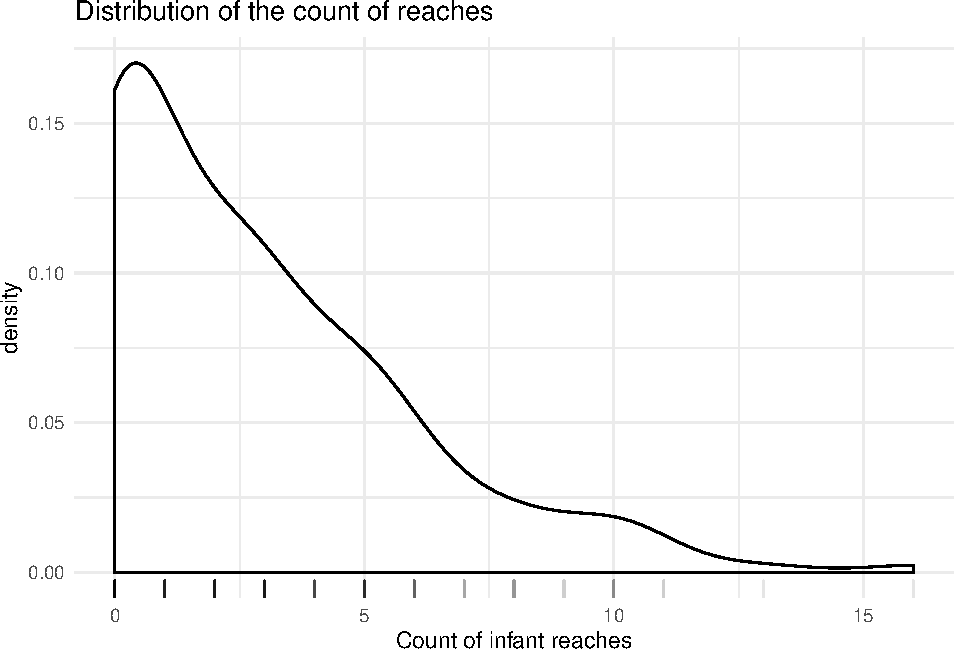
\includegraphics{supplement_files/figure-latex/reaches-1.pdf}

\begin{center}\rule{0.5\linewidth}{\linethickness}\end{center}

The following models test cultural group for infant reaches.

\begin{Shaded}
\begin{Highlighting}[]
\CommentTok{# Estimation of theta for the negbin() family}
\NormalTok{reach_nb <-}\StringTok{ }\KeywordTok{glm.nb}\NormalTok{(count }\OperatorTok{~}\StringTok{ }\NormalTok{months, }\DataTypeTok{data =}\NormalTok{ reach_tot)}
\NormalTok{theta <-}\StringTok{ }\KeywordTok{summary}\NormalTok{(reach_nb)[[}\StringTok{"theta"}\NormalTok{]]}

\NormalTok{reach_gam <-}\StringTok{ }\KeywordTok{gam}\NormalTok{(}
\NormalTok{  count }\OperatorTok{~}
\StringTok{    }\CommentTok{# parametric term}
\StringTok{    }\NormalTok{back_o }\OperatorTok{+}
\StringTok{    }\CommentTok{# reference smooth}
\StringTok{    }\KeywordTok{s}\NormalTok{(months, }\DataTypeTok{k =} \DecValTok{3}\NormalTok{) }\OperatorTok{+}
\StringTok{    }\CommentTok{# difference smoth}
\StringTok{    }\KeywordTok{s}\NormalTok{(months, }\DataTypeTok{k =} \DecValTok{3}\NormalTok{, }\DataTypeTok{by =}\NormalTok{ back_o) }\OperatorTok{+}
\StringTok{    }\CommentTok{# random smooths (random effect)}
\StringTok{    }\KeywordTok{s}\NormalTok{(months, dyad, }\DataTypeTok{k =} \DecValTok{2}\NormalTok{, }\DataTypeTok{bs =} \StringTok{"fs"}\NormalTok{, }\DataTypeTok{m =} \DecValTok{1}\NormalTok{),}
  \DataTypeTok{data =}\NormalTok{ reach_tot,}
  \DataTypeTok{method =} \StringTok{"ML"}\NormalTok{,}
  \DataTypeTok{family =} \KeywordTok{negbin}\NormalTok{(theta)}
\NormalTok{)}
\end{Highlighting}
\end{Shaded}

\begin{verbatim}
## Warning in gam.side(sm, X, tol = .Machine$double.eps^0.5): model has repeated 1-
## d smooths of same variable.
\end{verbatim}

\begin{Shaded}
\begin{Highlighting}[]
\KeywordTok{summary}\NormalTok{(reach_gam)}
\end{Highlighting}
\end{Shaded}

\begin{verbatim}
## 
## Family: Negative Binomial(0.936) 
## Link function: log 
## 
## Formula:
## count ~ back_o + s(months, k = 3) + s(months, k = 3, by = back_o) + 
##     s(months, dyad, k = 2, bs = "fs", m = 1)
## 
## Parametric coefficients:
##               Estimate Std. Error z value Pr(>|z|)   
## (Intercept)     0.5604     0.1945   2.882  0.00396 **
## back_oBengali   0.6600     0.2659   2.482  0.01305 * 
## back_oChinese   0.3094     0.2709   1.142  0.25336   
## ---
## Signif. codes:  0 '***' 0.001 '**' 0.01 '*' 0.05 '.' 0.1 ' ' 1
## 
## Approximate significance of smooth terms:
##                            edf  Ref.df Chi.sq p-value  
## s(months)                1.093   1.177  1.229  0.2704  
## s(months):back_oBengali  1.000   1.000  0.414  0.5200  
## s(months):back_oChinese  1.000   1.000  0.107  0.7439  
## s(months,dyad)          15.631 114.000 21.958  0.0243 *
## ---
## Signif. codes:  0 '***' 0.001 '**' 0.01 '*' 0.05 '.' 0.1 ' ' 1
## 
## R-sq.(adj) =  0.177   Deviance explained =   23%
## -ML = 381.91  Scale est. = 1         n = 176
\end{verbatim}

\begin{Shaded}
\begin{Highlighting}[]
\NormalTok{reach_gam_null <-}\StringTok{ }\KeywordTok{gam}\NormalTok{(}
\NormalTok{  count }\OperatorTok{~}
\StringTok{    }\CommentTok{# back_o +}
\StringTok{    }\KeywordTok{s}\NormalTok{(months, }\DataTypeTok{k =} \DecValTok{3}\NormalTok{) }\OperatorTok{+}
\StringTok{    }\CommentTok{# s(months, k = 3, by = back_o) +}
\StringTok{    }\KeywordTok{s}\NormalTok{(months, dyad, }\DataTypeTok{k =} \DecValTok{2}\NormalTok{, }\DataTypeTok{bs =} \StringTok{"fs"}\NormalTok{, }\DataTypeTok{m =} \DecValTok{1}\NormalTok{),}
  \DataTypeTok{data =}\NormalTok{ reach_tot,}
  \DataTypeTok{method =} \StringTok{"ML"}\NormalTok{,}
  \DataTypeTok{family =} \KeywordTok{negbin}\NormalTok{(theta)}
\NormalTok{)}
\end{Highlighting}
\end{Shaded}

\begin{verbatim}
## Warning in gam.side(sm, X, tol = .Machine$double.eps^0.5): model has repeated 1-
## d smooths of same variable.
\end{verbatim}

\begin{Shaded}
\begin{Highlighting}[]
\KeywordTok{compareML}\NormalTok{(reach_gam_null, reach_gam)}
\end{Highlighting}
\end{Shaded}

\begin{verbatim}
## reach_gam_null: count ~ s(months, k = 3) + s(months, dyad, k = 2, bs = "fs", 
##     m = 1)
## 
## reach_gam: count ~ back_o + s(months, k = 3) + s(months, k = 3, by = back_o) + 
##     s(months, dyad, k = 2, bs = "fs", m = 1)
## 
## Chi-square test of ML scores
## -----
##            Model   Score Edf Difference    Df p.value Sig.
## 1 reach_gam_null 385.168   5                              
## 2      reach_gam 381.907  11      3.261 6.000   0.367     
## 
## AIC difference: -0.70, model reach_gam_null has lower AIC.
\end{verbatim}

\begin{verbatim}
## Warning in compareML(reach_gam_null, reach_gam): Only small difference in ML...
\end{verbatim}

\begin{Shaded}
\begin{Highlighting}[]
\KeywordTok{plot_smooths}\NormalTok{(reach_gam, months, }\DataTypeTok{facet_terms =}\NormalTok{ back_o, }\DataTypeTok{series_length =} \DecValTok{25}\NormalTok{, }\DataTypeTok{transform =}\NormalTok{ exp) }\OperatorTok{+}
\StringTok{  }\KeywordTok{labs}\NormalTok{(}\DataTypeTok{x =} \StringTok{"Months"}\NormalTok{, }\DataTypeTok{y =} \StringTok{"Count of reaches"}\NormalTok{, }\DataTypeTok{title =} \StringTok{"Predicted development of reaches by background"}\NormalTok{)}
\end{Highlighting}
\end{Shaded}

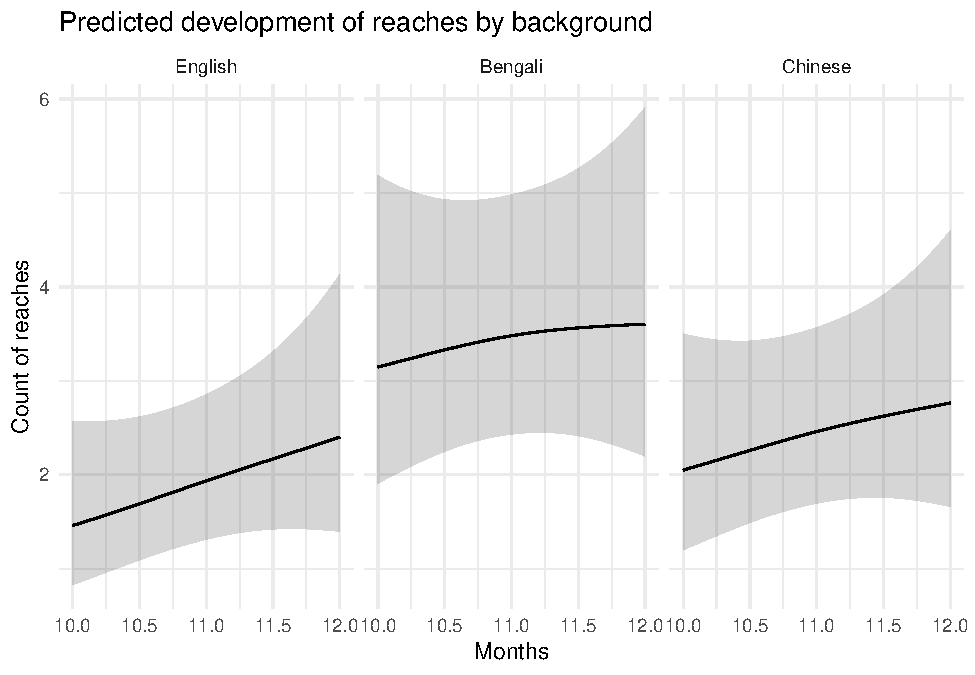
\includegraphics{supplement_files/figure-latex/reach-gam-plot-1.pdf}

\begin{center}\rule{0.5\linewidth}{\linethickness}\end{center}

The following models test the development of infant reaches.

\begin{Shaded}
\begin{Highlighting}[]
\NormalTok{reach_gam_}\DecValTok{2}\NormalTok{ <-}\StringTok{ }\KeywordTok{gam}\NormalTok{(}
\NormalTok{  count }\OperatorTok{~}
\StringTok{    }\KeywordTok{s}\NormalTok{(months, }\DataTypeTok{k =} \DecValTok{3}\NormalTok{) }\OperatorTok{+}
\StringTok{    }\KeywordTok{s}\NormalTok{(months, dyad, }\DataTypeTok{k =} \DecValTok{2}\NormalTok{, }\DataTypeTok{bs =} \StringTok{"fs"}\NormalTok{, }\DataTypeTok{m =} \DecValTok{1}\NormalTok{),}
  \DataTypeTok{data =}\NormalTok{ reach_tot,}
  \DataTypeTok{method =} \StringTok{"ML"}\NormalTok{,}
  \DataTypeTok{family =} \KeywordTok{negbin}\NormalTok{(theta)}
\NormalTok{)}
\end{Highlighting}
\end{Shaded}

\begin{verbatim}
## Warning in gam.side(sm, X, tol = .Machine$double.eps^0.5): model has repeated 1-
## d smooths of same variable.
\end{verbatim}

\begin{Shaded}
\begin{Highlighting}[]
\NormalTok{reach_gam_}\DecValTok{2}\NormalTok{_null <-}\StringTok{ }\KeywordTok{gam}\NormalTok{(}
\NormalTok{  count }\OperatorTok{~}
\StringTok{    }\CommentTok{# s(months, k = 3) +}
\StringTok{    }\KeywordTok{s}\NormalTok{(months, dyad, }\DataTypeTok{k =} \DecValTok{2}\NormalTok{, }\DataTypeTok{bs =} \StringTok{"fs"}\NormalTok{, }\DataTypeTok{m =} \DecValTok{1}\NormalTok{),}
  \DataTypeTok{data =}\NormalTok{ reach_tot,}
  \DataTypeTok{method =} \StringTok{"ML"}\NormalTok{,}
  \DataTypeTok{family =} \KeywordTok{negbin}\NormalTok{(theta)}
\NormalTok{)}
\KeywordTok{compareML}\NormalTok{(reach_gam_}\DecValTok{2}\NormalTok{_null, reach_gam_}\DecValTok{2}\NormalTok{)}
\end{Highlighting}
\end{Shaded}

\begin{verbatim}
## reach_gam_2_null: count ~ s(months, dyad, k = 2, bs = "fs", m = 1)
## 
## reach_gam_2: count ~ s(months, k = 3) + s(months, dyad, k = 2, bs = "fs", 
##     m = 1)
## 
## Chi-square test of ML scores
## -----
##              Model    Score Edf Difference    Df p.value Sig.
## 1 reach_gam_2_null 385.9817   3                              
## 2      reach_gam_2 385.1680   5      0.814 2.000   0.443     
## 
## AIC difference: -4.16, model reach_gam_2_null has lower AIC.
\end{verbatim}

\begin{verbatim}
## Warning in compareML(reach_gam_2_null, reach_gam_2): Only small difference in ML...
\end{verbatim}

\begin{Shaded}
\begin{Highlighting}[]
\KeywordTok{plot_smooths}\NormalTok{(reach_gam_}\DecValTok{2}\NormalTok{, months, }\DataTypeTok{series_length =} \DecValTok{25}\NormalTok{, }\DataTypeTok{transform =}\NormalTok{ exp) }\OperatorTok{+}
\StringTok{  }\KeywordTok{labs}\NormalTok{(}\DataTypeTok{x =} \StringTok{"Months"}\NormalTok{, }\DataTypeTok{y =} \StringTok{"Count of reaches"}\NormalTok{, }\DataTypeTok{title =} \StringTok{"Predicted development of reaches"}\NormalTok{)}
\end{Highlighting}
\end{Shaded}

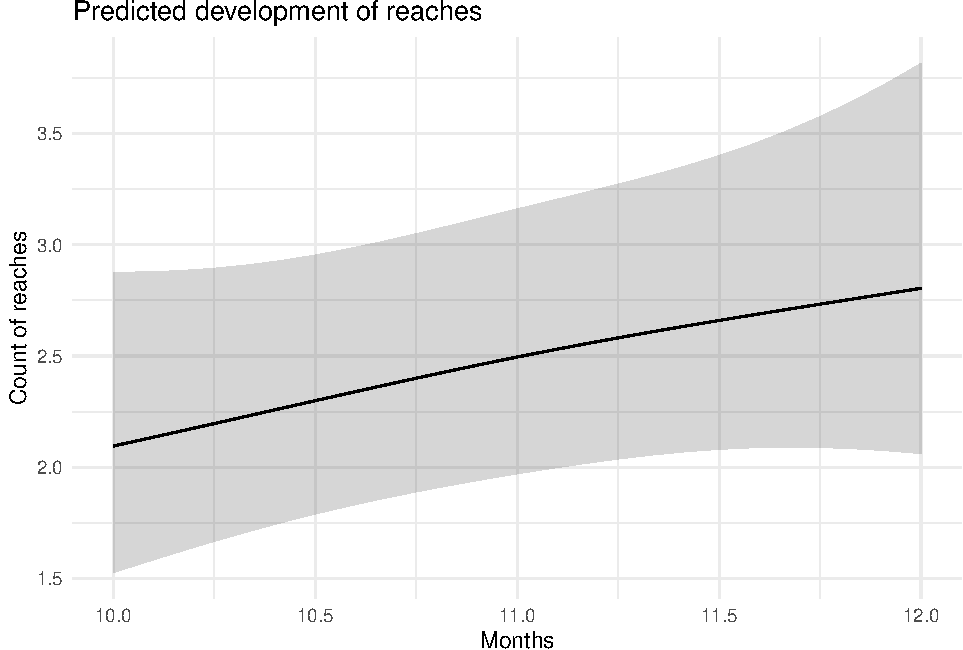
\includegraphics{supplement_files/figure-latex/reach-gam-2-plot-1.pdf}

\hypertarget{hgs-development}{%
\subsection{HGs development}\label{hgs-development}}

\begin{Shaded}
\begin{Highlighting}[]
\NormalTok{hg_tot }\OperatorTok
\StringTok{  }\KeywordTok{ggplot}\NormalTok{(}\KeywordTok{aes}\NormalTok{(count)) }\OperatorTok{+}\StringTok{ }\KeywordTok{geom_density}\NormalTok{() }\OperatorTok{+}\StringTok{ }\KeywordTok{geom_rug}\NormalTok{(}\DataTypeTok{alpha =} \FloatTok{0.1}\NormalTok{) }\OperatorTok{+}
\StringTok{  }\KeywordTok{labs}\NormalTok{(}
    \DataTypeTok{title =} \StringTok{"Distribution of the count of HoGs"}\NormalTok{,}
    \DataTypeTok{x =} \StringTok{"Count of infant HoGs"}
\NormalTok{  )}
\end{Highlighting}
\end{Shaded}

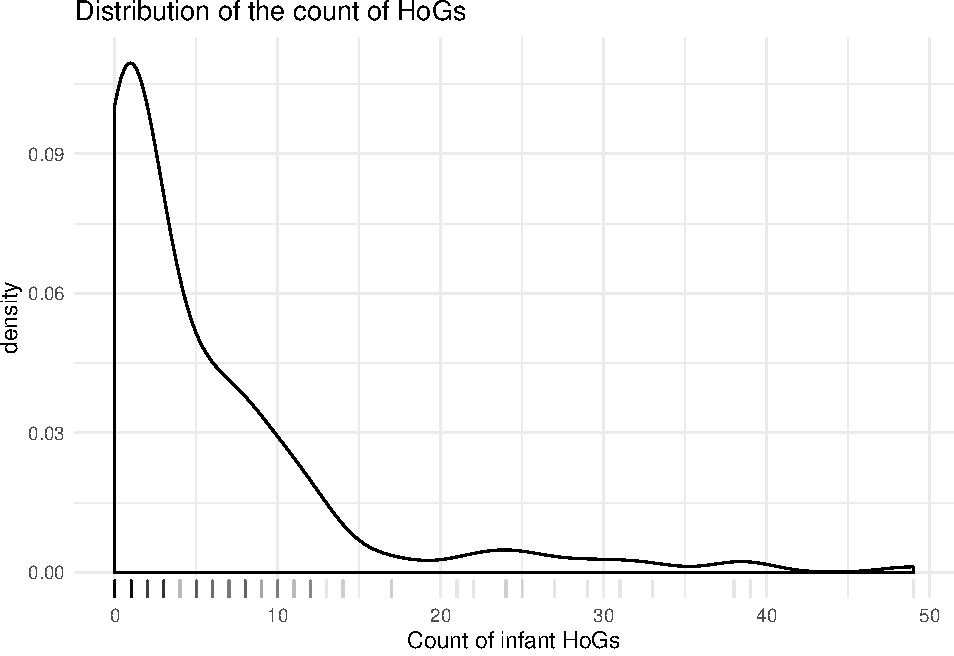
\includegraphics{supplement_files/figure-latex/hog-1.pdf}

\begin{center}\rule{0.5\linewidth}{\linethickness}\end{center}

The following models test cultural group differences for infant HoGs.

\begin{Shaded}
\begin{Highlighting}[]
\NormalTok{hg_nb <-}\StringTok{ }\KeywordTok{glm.nb}\NormalTok{(count }\OperatorTok{~}\StringTok{ }\NormalTok{months, }\DataTypeTok{data =}\NormalTok{ hg_tot)}
\NormalTok{theta_}\DecValTok{2}\NormalTok{ <-}\StringTok{ }\KeywordTok{summary}\NormalTok{(hg_nb)[[}\StringTok{"theta"}\NormalTok{]]}

\NormalTok{hg_gam <-}\StringTok{ }\KeywordTok{gam}\NormalTok{(}
\NormalTok{  count }\OperatorTok{~}
\StringTok{    }\NormalTok{back_o }\OperatorTok{+}
\StringTok{    }\KeywordTok{s}\NormalTok{(months, }\DataTypeTok{k =} \DecValTok{3}\NormalTok{) }\OperatorTok{+}
\StringTok{    }\KeywordTok{s}\NormalTok{(months, }\DataTypeTok{k =} \DecValTok{3}\NormalTok{, }\DataTypeTok{by =}\NormalTok{ back_o) }\OperatorTok{+}
\StringTok{    }\KeywordTok{s}\NormalTok{(months, dyad, }\DataTypeTok{k =} \DecValTok{2}\NormalTok{, }\DataTypeTok{bs =} \StringTok{"fs"}\NormalTok{, }\DataTypeTok{m =} \DecValTok{1}\NormalTok{),}
  \DataTypeTok{data =}\NormalTok{ hg_tot,}
  \DataTypeTok{method =} \StringTok{"ML"}\NormalTok{,}
  \DataTypeTok{family =} \KeywordTok{negbin}\NormalTok{(theta_}\DecValTok{2}\NormalTok{)}
\NormalTok{)}
\end{Highlighting}
\end{Shaded}

\begin{verbatim}
## Warning in gam.side(sm, X, tol = .Machine$double.eps^0.5): model has repeated 1-
## d smooths of same variable.
\end{verbatim}

\begin{Shaded}
\begin{Highlighting}[]
\KeywordTok{summary}\NormalTok{(hg_gam)}
\end{Highlighting}
\end{Shaded}

\begin{verbatim}
## 
## Family: Negative Binomial(0.639) 
## Link function: log 
## 
## Formula:
## count ~ back_o + s(months, k = 3) + s(months, k = 3, by = back_o) + 
##     s(months, dyad, k = 2, bs = "fs", m = 1)
## 
## Parametric coefficients:
##               Estimate Std. Error z value Pr(>|z|)   
## (Intercept)     0.7182     0.2261   3.176  0.00149 **
## back_oBengali   0.9442     0.3102   3.044  0.00234 **
## back_oChinese   0.7602     0.3122   2.435  0.01489 * 
## ---
## Signif. codes:  0 '***' 0.001 '**' 0.01 '*' 0.05 '.' 0.1 ' ' 1
## 
## Approximate significance of smooth terms:
##                           edf Ref.df Chi.sq p-value   
## s(months)                1.00      1  9.689 0.00185 **
## s(months):back_oBengali  1.00      1  0.012 0.91440   
## s(months):back_oChinese  1.00      1  0.370 0.54295   
## s(months,dyad)          17.73    114 26.141 0.01168 * 
## ---
## Signif. codes:  0 '***' 0.001 '**' 0.01 '*' 0.05 '.' 0.1 ' ' 1
## 
## R-sq.(adj) =  0.335   Deviance explained = 38.6%
## -ML = 455.97  Scale est. = 1         n = 176
\end{verbatim}

\begin{Shaded}
\begin{Highlighting}[]
\NormalTok{hg_gam_null <-}\StringTok{ }\KeywordTok{gam}\NormalTok{(}
\NormalTok{  count }\OperatorTok{~}
\StringTok{    }\CommentTok{# back_o +}
\StringTok{    }\KeywordTok{s}\NormalTok{(months, }\DataTypeTok{k =} \DecValTok{3}\NormalTok{) }\OperatorTok{+}
\StringTok{    }\CommentTok{# s(months, k = 3, by = back_o) +}
\StringTok{    }\KeywordTok{s}\NormalTok{(months, dyad, }\DataTypeTok{k =} \DecValTok{2}\NormalTok{, }\DataTypeTok{bs =} \StringTok{"fs"}\NormalTok{, }\DataTypeTok{m =} \DecValTok{1}\NormalTok{),}
  \DataTypeTok{data =}\NormalTok{ hg_tot,}
  \DataTypeTok{method =} \StringTok{"ML"}\NormalTok{,}
  \DataTypeTok{family =} \KeywordTok{negbin}\NormalTok{(theta_}\DecValTok{2}\NormalTok{)}
\NormalTok{)}
\end{Highlighting}
\end{Shaded}

\begin{verbatim}
## Warning in gam.side(sm, X, tol = .Machine$double.eps^0.5): model has repeated 1-
## d smooths of same variable.
\end{verbatim}

\begin{Shaded}
\begin{Highlighting}[]
\KeywordTok{compareML}\NormalTok{(hg_gam_null, hg_gam)}
\end{Highlighting}
\end{Shaded}

\begin{verbatim}
## hg_gam_null: count ~ s(months, k = 3) + s(months, dyad, k = 2, bs = "fs", 
##     m = 1)
## 
## hg_gam: count ~ back_o + s(months, k = 3) + s(months, k = 3, by = back_o) + 
##     s(months, dyad, k = 2, bs = "fs", m = 1)
## 
## Chi-square test of ML scores
## -----
##         Model    Score Edf Difference    Df p.value Sig.
## 1 hg_gam_null 460.7010   5                              
## 2      hg_gam 455.9701  11      4.731 6.000   0.149     
## 
## AIC difference: -1.78, model hg_gam_null has lower AIC.
\end{verbatim}

\begin{verbatim}
## Warning in compareML(hg_gam_null, hg_gam): Only small difference in ML...
\end{verbatim}

\begin{Shaded}
\begin{Highlighting}[]
\KeywordTok{plot_smooths}\NormalTok{(hg_gam, months, }\DataTypeTok{facet_terms =}\NormalTok{ back_o, }\DataTypeTok{series_length =} \DecValTok{25}\NormalTok{, }\DataTypeTok{transform =}\NormalTok{ exp) }\OperatorTok{+}
\StringTok{  }\KeywordTok{labs}\NormalTok{(}\DataTypeTok{x =} \StringTok{"Months"}\NormalTok{, }\DataTypeTok{y =} \StringTok{"Count of HoGs"}\NormalTok{, }\DataTypeTok{title =} \StringTok{"Predicted development of HoGs by background"}\NormalTok{)}
\end{Highlighting}
\end{Shaded}

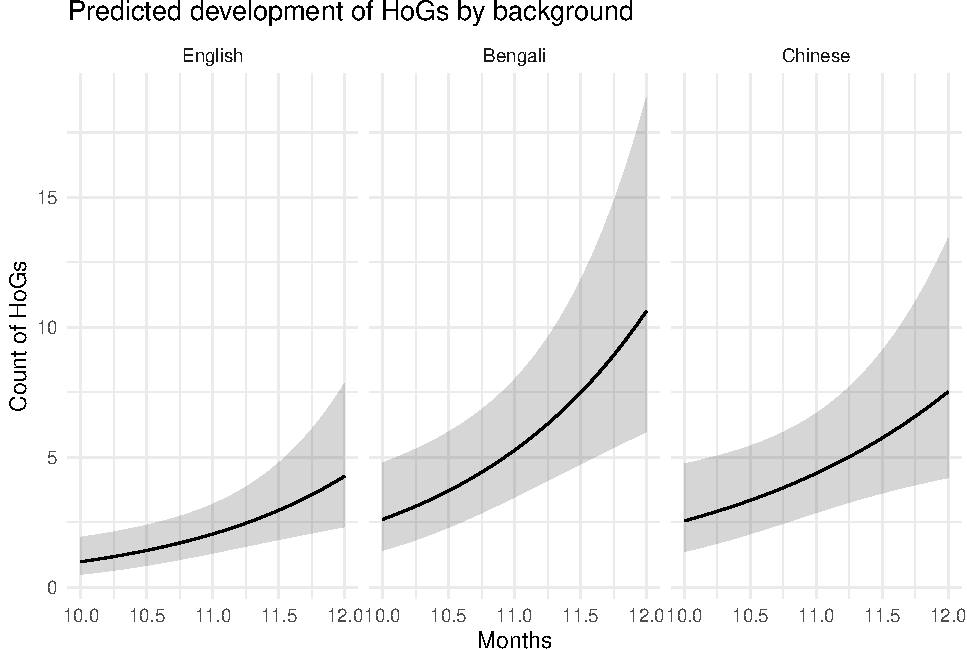
\includegraphics{supplement_files/figure-latex/hg-gam-plot-1.pdf}

\begin{center}\rule{0.5\linewidth}{\linethickness}\end{center}

The following models test development of infant HoGs.

\begin{Shaded}
\begin{Highlighting}[]
\NormalTok{hg_gam_}\DecValTok{2}\NormalTok{ <-}\StringTok{ }\KeywordTok{gam}\NormalTok{(}
\NormalTok{  count }\OperatorTok{~}
\StringTok{    }\KeywordTok{s}\NormalTok{(months, }\DataTypeTok{k =} \DecValTok{3}\NormalTok{) }\OperatorTok{+}
\StringTok{    }\KeywordTok{s}\NormalTok{(months, dyad, }\DataTypeTok{k =} \DecValTok{2}\NormalTok{, }\DataTypeTok{bs =} \StringTok{"fs"}\NormalTok{, }\DataTypeTok{m =} \DecValTok{1}\NormalTok{),}
  \DataTypeTok{data =}\NormalTok{ hg_tot,}
  \DataTypeTok{method =} \StringTok{"ML"}\NormalTok{,}
  \DataTypeTok{family =} \KeywordTok{negbin}\NormalTok{(theta_}\DecValTok{2}\NormalTok{)}
\NormalTok{)}
\end{Highlighting}
\end{Shaded}

\begin{verbatim}
## Warning in gam.side(sm, X, tol = .Machine$double.eps^0.5): model has repeated 1-
## d smooths of same variable.
\end{verbatim}

\begin{Shaded}
\begin{Highlighting}[]
\NormalTok{hg_gam_}\DecValTok{2}\NormalTok{_null <-}\StringTok{ }\KeywordTok{gam}\NormalTok{(}
\NormalTok{  count }\OperatorTok{~}
\StringTok{    }\CommentTok{# s(months, k = 3) +}
\StringTok{    }\KeywordTok{s}\NormalTok{(months, dyad, }\DataTypeTok{k =} \DecValTok{2}\NormalTok{, }\DataTypeTok{bs =} \StringTok{"fs"}\NormalTok{, }\DataTypeTok{m =} \DecValTok{1}\NormalTok{),}
  \DataTypeTok{data =}\NormalTok{ hg_tot,}
  \DataTypeTok{method =} \StringTok{"ML"}\NormalTok{,}
  \DataTypeTok{family =} \KeywordTok{negbin}\NormalTok{(theta_}\DecValTok{2}\NormalTok{)}
\NormalTok{)}
\KeywordTok{compareML}\NormalTok{(hg_gam_}\DecValTok{2}\NormalTok{_null, hg_gam_}\DecValTok{2}\NormalTok{)}
\end{Highlighting}
\end{Shaded}

\begin{verbatim}
## hg_gam_2_null: count ~ s(months, dyad, k = 2, bs = "fs", m = 1)
## 
## hg_gam_2: count ~ s(months, k = 3) + s(months, dyad, k = 2, bs = "fs", 
##     m = 1)
## 
## Chi-square test of ML scores
## -----
##           Model    Score Edf Difference    Df   p.value Sig.
## 1 hg_gam_2_null 473.0614   3                                
## 2      hg_gam_2 460.7010   5     12.360 2.000 4.285e-06  ***
## 
## AIC difference: 24.45, model hg_gam_2 has lower AIC.
\end{verbatim}

\begin{Shaded}
\begin{Highlighting}[]
\KeywordTok{plot_smooths}\NormalTok{(hg_gam_}\DecValTok{2}\NormalTok{, months, }\DataTypeTok{series_length =} \DecValTok{25}\NormalTok{, }\DataTypeTok{transform =}\NormalTok{ exp) }\OperatorTok{+}
\StringTok{  }\KeywordTok{labs}\NormalTok{(}\DataTypeTok{x =} \StringTok{"Months"}\NormalTok{, }\DataTypeTok{y =} \StringTok{"Count of HoGs"}\NormalTok{, }\DataTypeTok{title =} \StringTok{"Predicted development of HoGs"}\NormalTok{)}
\end{Highlighting}
\end{Shaded}

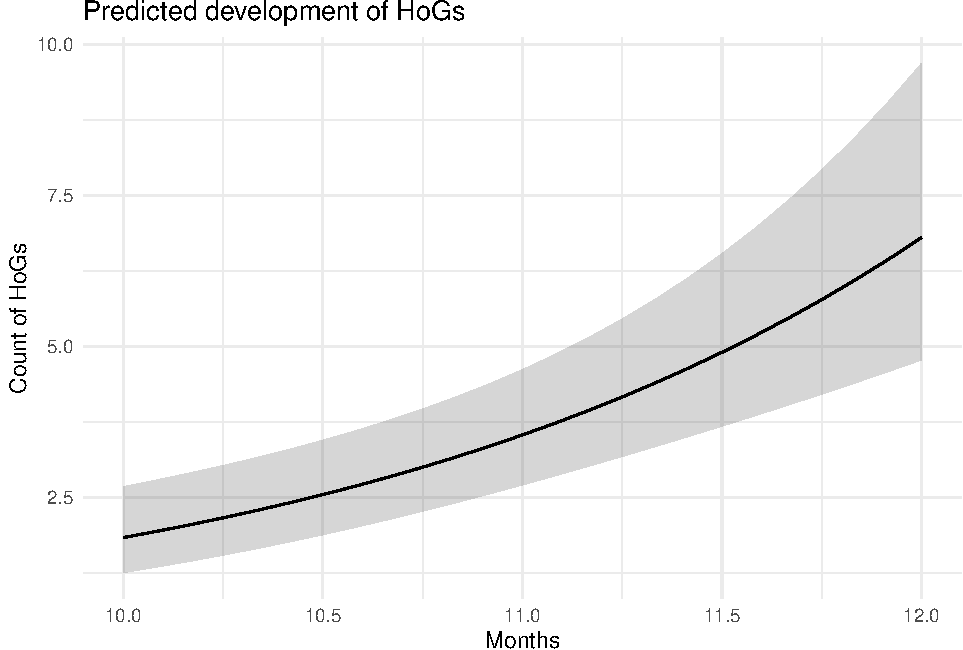
\includegraphics{supplement_files/figure-latex/hg-gam-2-plot-1.pdf}

\hypertarget{points-development}{%
\subsection{Points development}\label{points-development}}

\begin{Shaded}
\begin{Highlighting}[]
\NormalTok{point_tot }\OperatorTok
\StringTok{  }\KeywordTok{ggplot}\NormalTok{(}\KeywordTok{aes}\NormalTok{(count)) }\OperatorTok{+}\StringTok{ }\KeywordTok{geom_density}\NormalTok{() }\OperatorTok{+}\StringTok{ }\KeywordTok{geom_rug}\NormalTok{(}\DataTypeTok{alpha =} \FloatTok{0.1}\NormalTok{) }\OperatorTok{+}
\StringTok{  }\KeywordTok{labs}\NormalTok{(}
    \DataTypeTok{title =} \StringTok{"Distribution of the count of points"}\NormalTok{,}
    \DataTypeTok{x =} \StringTok{"Count of infant points"}
\NormalTok{  )}
\end{Highlighting}
\end{Shaded}

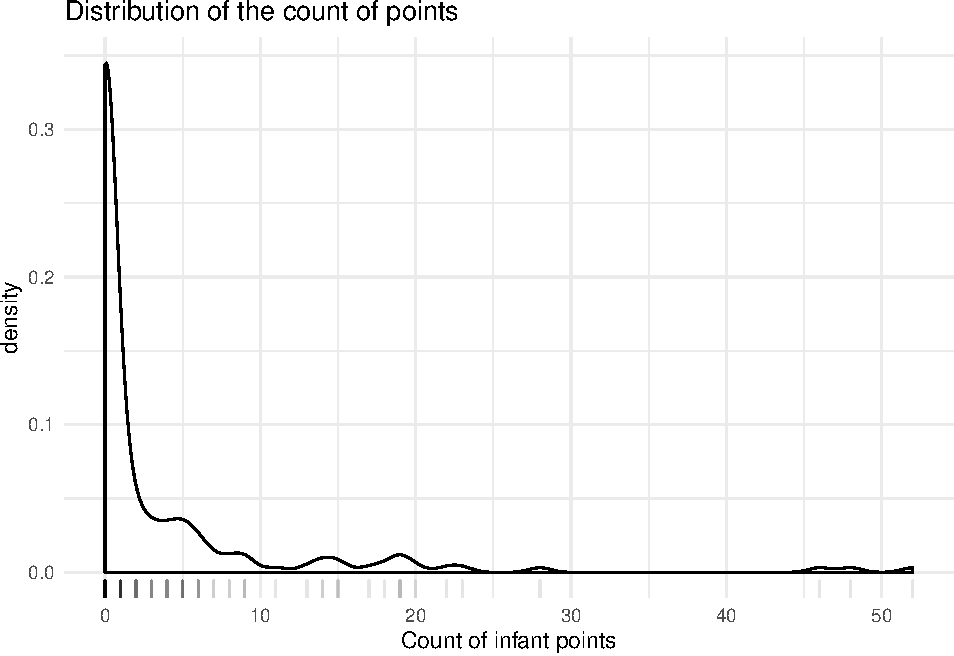
\includegraphics{supplement_files/figure-latex/points-1.pdf}

\begin{center}\rule{0.5\linewidth}{\linethickness}\end{center}

The following models test cultural group differences in infant pointing.

\begin{Shaded}
\begin{Highlighting}[]
\NormalTok{point_nb <-}\StringTok{ }\KeywordTok{glm.nb}\NormalTok{(count }\OperatorTok{~}\StringTok{ }\NormalTok{months, }\DataTypeTok{data =}\NormalTok{ point_tot)}
\NormalTok{theta_}\DecValTok{3}\NormalTok{ <-}\StringTok{ }\KeywordTok{summary}\NormalTok{(point_nb)[[}\StringTok{"theta"}\NormalTok{]]}

\NormalTok{point_gam <-}\StringTok{ }\KeywordTok{gam}\NormalTok{(}
\NormalTok{  count }\OperatorTok{~}
\StringTok{    }\NormalTok{back_o }\OperatorTok{+}
\StringTok{    }\KeywordTok{s}\NormalTok{(months, }\DataTypeTok{k =} \DecValTok{3}\NormalTok{) }\OperatorTok{+}
\StringTok{    }\KeywordTok{s}\NormalTok{(months, }\DataTypeTok{k =} \DecValTok{3}\NormalTok{, }\DataTypeTok{by =}\NormalTok{ back_o) }\OperatorTok{+}
\StringTok{    }\KeywordTok{s}\NormalTok{(months, dyad, }\DataTypeTok{k =} \DecValTok{2}\NormalTok{, }\DataTypeTok{bs =} \StringTok{"fs"}\NormalTok{, }\DataTypeTok{m =} \DecValTok{1}\NormalTok{),}
  \DataTypeTok{data =}\NormalTok{ point_tot,}
  \DataTypeTok{method =} \StringTok{"ML"}\NormalTok{,}
  \DataTypeTok{family =} \KeywordTok{negbin}\NormalTok{(theta_}\DecValTok{3}\NormalTok{)}
\NormalTok{)}
\end{Highlighting}
\end{Shaded}

\begin{verbatim}
## Warning in gam.side(sm, X, tol = .Machine$double.eps^0.5): model has repeated 1-
## d smooths of same variable.
\end{verbatim}

\begin{Shaded}
\begin{Highlighting}[]
\KeywordTok{summary}\NormalTok{(point_gam)}
\end{Highlighting}
\end{Shaded}

\begin{verbatim}
## 
## Family: Negative Binomial(0.19) 
## Link function: log 
## 
## Formula:
## count ~ back_o + s(months, k = 3) + s(months, k = 3, by = back_o) + 
##     s(months, dyad, k = 2, bs = "fs", m = 1)
## 
## Parametric coefficients:
##               Estimate Std. Error z value Pr(>|z|)
## (Intercept)     0.5860     0.3926   1.492    0.136
## back_oBengali  -0.4005     0.5611  -0.714    0.475
## back_oChinese  -0.4788     0.5701  -0.840    0.401
## 
## Approximate significance of smooth terms:
##                            edf  Ref.df Chi.sq p-value  
## s(months)                1.000   1.000  1.096  0.2952  
## s(months):back_oBengali  1.529   1.777  0.689  0.5834  
## s(months):back_oChinese  1.000   1.000  2.118  0.1456  
## s(months,dyad)          18.927 114.000 26.889  0.0205 *
## ---
## Signif. codes:  0 '***' 0.001 '**' 0.01 '*' 0.05 '.' 0.1 ' ' 1
## 
## R-sq.(adj) =  0.327   Deviance explained = 41.3%
## -ML = 328.06  Scale est. = 1         n = 176
\end{verbatim}

\begin{Shaded}
\begin{Highlighting}[]
\NormalTok{point_gam_null <-}\StringTok{ }\KeywordTok{gam}\NormalTok{(}
\NormalTok{  count }\OperatorTok{~}
\StringTok{    }\CommentTok{# back_o +}
\StringTok{    }\KeywordTok{s}\NormalTok{(months, }\DataTypeTok{k =} \DecValTok{3}\NormalTok{) }\OperatorTok{+}
\StringTok{    }\CommentTok{# s(months, k = 3, by = back_o) +}
\StringTok{    }\KeywordTok{s}\NormalTok{(months, dyad, }\DataTypeTok{k =} \DecValTok{2}\NormalTok{, }\DataTypeTok{bs =} \StringTok{"fs"}\NormalTok{, }\DataTypeTok{m =} \DecValTok{1}\NormalTok{),}
  \DataTypeTok{data =}\NormalTok{ point_tot,}
  \DataTypeTok{method =} \StringTok{"ML"}\NormalTok{,}
  \DataTypeTok{family =} \KeywordTok{negbin}\NormalTok{(theta_}\DecValTok{3}\NormalTok{)}
\NormalTok{)}
\end{Highlighting}
\end{Shaded}

\begin{verbatim}
## Warning in gam.side(sm, X, tol = .Machine$double.eps^0.5): model has repeated 1-
## d smooths of same variable.
\end{verbatim}

\begin{Shaded}
\begin{Highlighting}[]
\KeywordTok{compareML}\NormalTok{(point_gam_null, point_gam)}
\end{Highlighting}
\end{Shaded}

\begin{verbatim}
## point_gam_null: count ~ s(months, k = 3) + s(months, dyad, k = 2, bs = "fs", 
##     m = 1)
## 
## point_gam: count ~ back_o + s(months, k = 3) + s(months, k = 3, by = back_o) + 
##     s(months, dyad, k = 2, bs = "fs", m = 1)
## 
## Chi-square test of ML scores
## -----
##            Model    Score Edf Difference    Df p.value Sig.
## 1 point_gam_null 329.5969   5                              
## 2      point_gam 328.0561  11      1.541 6.000   0.799     
## 
## AIC difference: -7.63, model point_gam_null has lower AIC.
\end{verbatim}

\begin{verbatim}
## Warning in compareML(point_gam_null, point_gam): Only small difference in ML...
\end{verbatim}

\begin{Shaded}
\begin{Highlighting}[]
\KeywordTok{plot_smooths}\NormalTok{(point_gam, months, }\DataTypeTok{facet_terms =}\NormalTok{ back_o, }\DataTypeTok{series_length =} \DecValTok{25}\NormalTok{, }\DataTypeTok{transform =}\NormalTok{ exp) }\OperatorTok{+}
\StringTok{  }\KeywordTok{labs}\NormalTok{(}\DataTypeTok{x =} \StringTok{"Months"}\NormalTok{, }\DataTypeTok{y =} \StringTok{"Count of points"}\NormalTok{, }\DataTypeTok{title =} \StringTok{"Predicted development of points by background"}\NormalTok{)}
\end{Highlighting}
\end{Shaded}

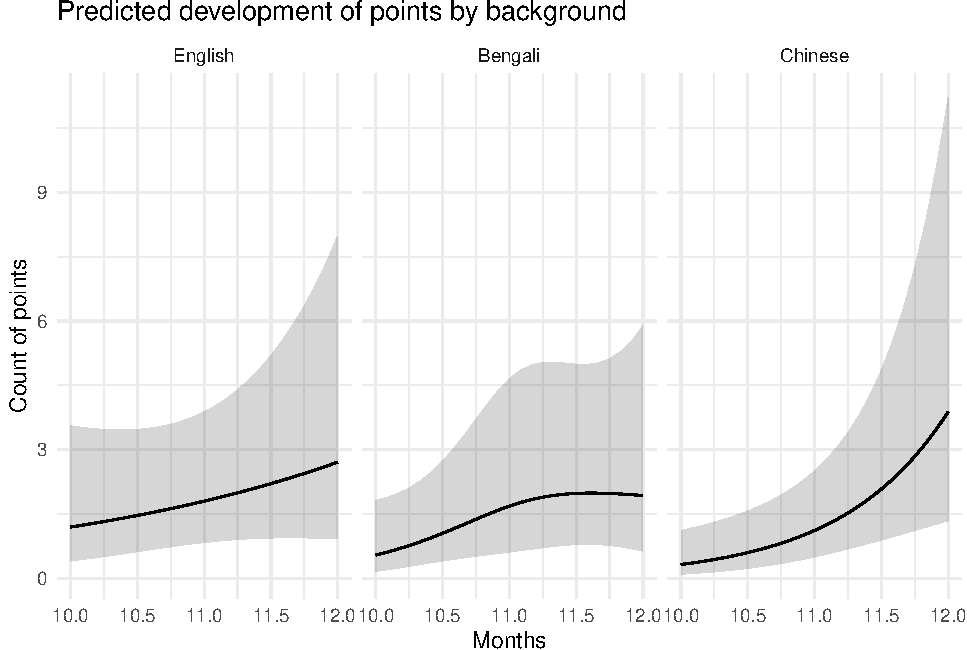
\includegraphics{supplement_files/figure-latex/point-gam-plot-1.pdf}

\begin{center}\rule{0.5\linewidth}{\linethickness}\end{center}

The following models test development of infant pointing.

\begin{Shaded}
\begin{Highlighting}[]
\NormalTok{point_gam_}\DecValTok{2}\NormalTok{ <-}\StringTok{ }\KeywordTok{gam}\NormalTok{(}
\NormalTok{  count }\OperatorTok{~}
\StringTok{    }\KeywordTok{s}\NormalTok{(months, }\DataTypeTok{k =} \DecValTok{3}\NormalTok{) }\OperatorTok{+}
\StringTok{    }\KeywordTok{s}\NormalTok{(months, dyad, }\DataTypeTok{k =} \DecValTok{2}\NormalTok{, }\DataTypeTok{bs =} \StringTok{"fs"}\NormalTok{, }\DataTypeTok{m =} \DecValTok{1}\NormalTok{),}
  \DataTypeTok{data =}\NormalTok{ point_tot,}
  \DataTypeTok{method =} \StringTok{"ML"}\NormalTok{,}
  \DataTypeTok{family =} \KeywordTok{negbin}\NormalTok{(theta_}\DecValTok{3}\NormalTok{)}
\NormalTok{)}
\end{Highlighting}
\end{Shaded}

\begin{verbatim}
## Warning in gam.side(sm, X, tol = .Machine$double.eps^0.5): model has repeated 1-
## d smooths of same variable.
\end{verbatim}

\begin{Shaded}
\begin{Highlighting}[]
\NormalTok{point_gam_}\DecValTok{2}\NormalTok{_null <-}\StringTok{ }\KeywordTok{gam}\NormalTok{(}
\NormalTok{  count }\OperatorTok{~}
\StringTok{    }\CommentTok{# s(months, k = 3) +}
\StringTok{    }\KeywordTok{s}\NormalTok{(months, dyad, }\DataTypeTok{k =} \DecValTok{2}\NormalTok{, }\DataTypeTok{bs =} \StringTok{"fs"}\NormalTok{, }\DataTypeTok{m =} \DecValTok{1}\NormalTok{),}
  \DataTypeTok{data =}\NormalTok{ point_tot,}
  \DataTypeTok{method =} \StringTok{"ML"}\NormalTok{,}
  \DataTypeTok{family =} \KeywordTok{negbin}\NormalTok{(theta_}\DecValTok{3}\NormalTok{)}
\NormalTok{)}
\KeywordTok{compareML}\NormalTok{(point_gam_}\DecValTok{2}\NormalTok{_null, point_gam_}\DecValTok{2}\NormalTok{)}
\end{Highlighting}
\end{Shaded}

\begin{verbatim}
## point_gam_2_null: count ~ s(months, dyad, k = 2, bs = "fs", m = 1)
## 
## point_gam_2: count ~ s(months, k = 3) + s(months, dyad, k = 2, bs = "fs", 
##     m = 1)
## 
## Chi-square test of ML scores
## -----
##              Model    Score Edf Difference    Df p.value Sig.
## 1 point_gam_2_null 334.1818   3                              
## 2      point_gam_2 329.5969   5      4.585 2.000   0.010  *  
## 
## AIC difference: 10.11, model point_gam_2 has lower AIC.
\end{verbatim}

\begin{verbatim}
## Warning in compareML(point_gam_2_null, point_gam_2): Only small difference in ML...
\end{verbatim}

\begin{Shaded}
\begin{Highlighting}[]
\KeywordTok{plot_smooths}\NormalTok{(point_gam_}\DecValTok{2}\NormalTok{, months, }\DataTypeTok{series_length =} \DecValTok{25}\NormalTok{, }\DataTypeTok{transform =}\NormalTok{ exp) }\OperatorTok{+}
\StringTok{  }\KeywordTok{labs}\NormalTok{(}\DataTypeTok{x =} \StringTok{"Months"}\NormalTok{, }\DataTypeTok{y =} \StringTok{"Count of points"}\NormalTok{, }\DataTypeTok{title =} \StringTok{"Predicted development of points"}\NormalTok{)}
\end{Highlighting}
\end{Shaded}

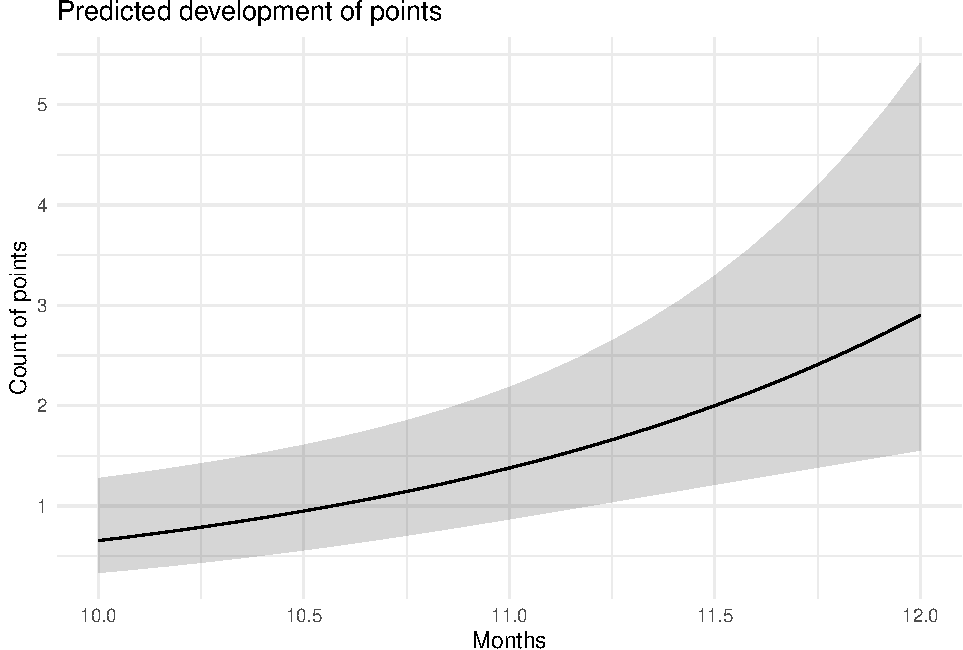
\includegraphics{supplement_files/figure-latex/point-gam-2-plot-1.pdf}

\newpage

\hypertarget{analysis-1b.-frequency-of-maternal-utterances-and-contingent-talk-to-infants-aged-10-12-months.}{%
\section{Analysis 1b. Frequency of maternal utterances and contingent
talk to infants aged 10-12
months.}\label{analysis-1b.-frequency-of-maternal-utterances-and-contingent-talk-to-infants-aged-10-12-months.}}

For maternal utterances we used a normal distribution, since the
distribution of the data was almost normal. For maternal contingent
talks instead we used again the negative binomial distribution for the
same reasons as above.

\hypertarget{maternal-utterances-development}{%
\subsection{Maternal utterances
development}\label{maternal-utterances-development}}

\begin{Shaded}
\begin{Highlighting}[]
\NormalTok{utterances_tot }\OperatorTok
\StringTok{  }\KeywordTok{ggplot}\NormalTok{(}\KeywordTok{aes}\NormalTok{(utterances)) }\OperatorTok{+}\StringTok{ }\KeywordTok{geom_density}\NormalTok{() }\OperatorTok{+}\StringTok{ }\KeywordTok{geom_rug}\NormalTok{(}\DataTypeTok{alpha =} \FloatTok{0.1}\NormalTok{) }\OperatorTok{+}
\StringTok{  }\KeywordTok{labs}\NormalTok{(}
    \DataTypeTok{title =} \StringTok{"Distribution of the count of utterances"}\NormalTok{,}
    \DataTypeTok{x =} \StringTok{"Count of maternal utterances"}
\NormalTok{  )}
\end{Highlighting}
\end{Shaded}

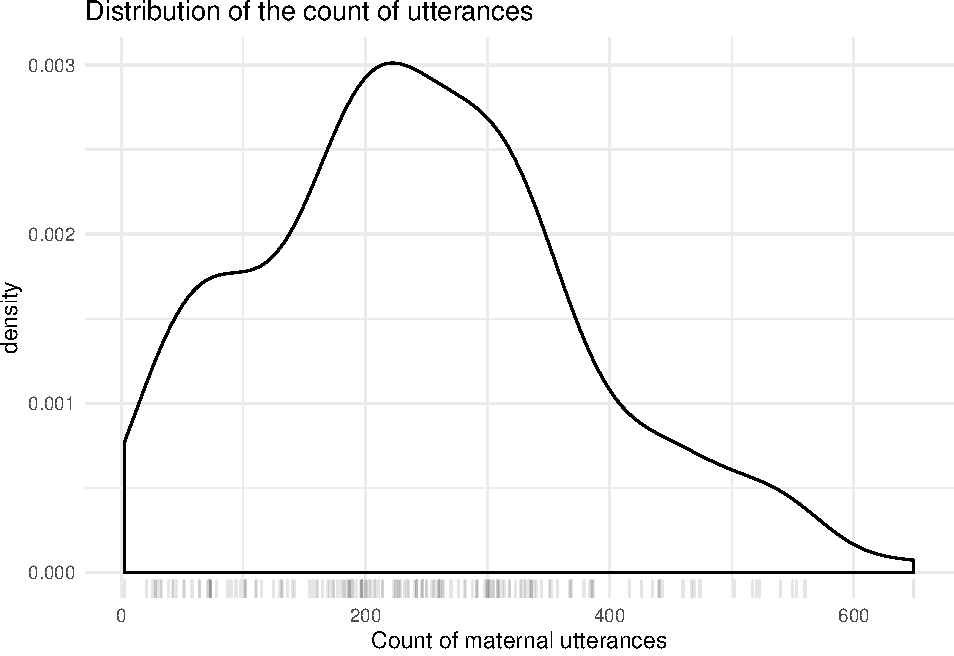
\includegraphics{supplement_files/figure-latex/utterances-1.pdf}

\begin{center}\rule{0.5\linewidth}{\linethickness}\end{center}

The following models test cultural group.

\begin{Shaded}
\begin{Highlighting}[]
\NormalTok{utter_gam <-}\StringTok{ }\KeywordTok{gam}\NormalTok{(}
\NormalTok{  utterances }\OperatorTok{~}
\StringTok{    }\NormalTok{back_o }\OperatorTok{+}
\StringTok{    }\KeywordTok{s}\NormalTok{(months, }\DataTypeTok{k =} \DecValTok{3}\NormalTok{) }\OperatorTok{+}
\StringTok{    }\KeywordTok{s}\NormalTok{(months, }\DataTypeTok{k =} \DecValTok{3}\NormalTok{, }\DataTypeTok{by =}\NormalTok{ back_o) }\OperatorTok{+}
\StringTok{    }\KeywordTok{s}\NormalTok{(months, dyad, }\DataTypeTok{k =} \DecValTok{2}\NormalTok{, }\DataTypeTok{bs =} \StringTok{"fs"}\NormalTok{, }\DataTypeTok{m =} \DecValTok{1}\NormalTok{),}
  \DataTypeTok{data =}\NormalTok{ utterances_tot,}
  \DataTypeTok{method =} \StringTok{"ML"}
\NormalTok{)}
\end{Highlighting}
\end{Shaded}

\begin{verbatim}
## Warning in gam.side(sm, X, tol = .Machine$double.eps^0.5): model has repeated 1-
## d smooths of same variable.
\end{verbatim}

\begin{Shaded}
\begin{Highlighting}[]
\KeywordTok{summary}\NormalTok{(utter_gam)}
\end{Highlighting}
\end{Shaded}

\begin{verbatim}
## 
## Family: gaussian 
## Link function: identity 
## 
## Formula:
## utterances ~ back_o + s(months, k = 3) + s(months, k = 3, by = back_o) + 
##     s(months, dyad, k = 2, bs = "fs", m = 1)
## 
## Parametric coefficients:
##               Estimate Std. Error t value Pr(>|t|)    
## (Intercept)     273.12      26.96  10.131   <2e-16 ***
## back_oBengali   -54.18      38.11  -1.422    0.159    
## back_oChinese   -26.50      38.03  -0.697    0.488    
## ---
## Signif. codes:  0 '***' 0.001 '**' 0.01 '*' 0.05 '.' 0.1 ' ' 1
## 
## Approximate significance of smooth terms:
##                            edf  Ref.df     F p-value    
## s(months)                1.712   1.894 1.087  0.2861    
## s(months):back_oBengali  1.001   1.001 1.303  0.2568    
## s(months):back_oChinese  1.318   1.513 2.269  0.0814 .  
## s(months,dyad)          75.684 113.000 7.557  <2e-16 ***
## ---
## Signif. codes:  0 '***' 0.001 '**' 0.01 '*' 0.05 '.' 0.1 ' ' 1
## 
## R-sq.(adj) =  0.843   Deviance explained = 91.9%
## -ML = 1010.1  Scale est. = 2773.3    n = 170
\end{verbatim}

\begin{Shaded}
\begin{Highlighting}[]
\NormalTok{utter_gam_null <-}\StringTok{ }\KeywordTok{gam}\NormalTok{(}
\NormalTok{  utterances }\OperatorTok{~}
\StringTok{    }\CommentTok{# back_o +}
\StringTok{    }\KeywordTok{s}\NormalTok{(months, }\DataTypeTok{k =} \DecValTok{3}\NormalTok{) }\OperatorTok{+}
\StringTok{    }\CommentTok{# s(months, k = 3, by = back_o) +}
\StringTok{    }\KeywordTok{s}\NormalTok{(months, dyad, }\DataTypeTok{k =} \DecValTok{2}\NormalTok{, }\DataTypeTok{bs =} \StringTok{"fs"}\NormalTok{, }\DataTypeTok{m =} \DecValTok{1}\NormalTok{),}
  \DataTypeTok{data =}\NormalTok{ utterances_tot,}
  \DataTypeTok{method =} \StringTok{"ML"}
\NormalTok{)}
\end{Highlighting}
\end{Shaded}

\begin{verbatim}
## Warning in gam.side(sm, X, tol = .Machine$double.eps^0.5): model has repeated 1-
## d smooths of same variable.
\end{verbatim}

\begin{Shaded}
\begin{Highlighting}[]
\KeywordTok{compareML}\NormalTok{(utter_gam_null, utter_gam)}
\end{Highlighting}
\end{Shaded}

\begin{verbatim}
## utter_gam_null: utterances ~ s(months, k = 3) + s(months, dyad, k = 2, bs = "fs", 
##     m = 1)
## 
## utter_gam: utterances ~ back_o + s(months, k = 3) + s(months, k = 3, by = back_o) + 
##     s(months, dyad, k = 2, bs = "fs", m = 1)
## 
## Chi-square test of ML scores
## -----
##            Model    Score Edf Difference    Df p.value Sig.
## 1 utter_gam_null 1013.245   5                              
## 2      utter_gam 1010.123  11      3.122 6.000   0.396     
## 
## AIC difference: -3.62, model utter_gam_null has lower AIC.
\end{verbatim}

\begin{verbatim}
## Warning in compareML(utter_gam_null, utter_gam): Only small difference in ML...
\end{verbatim}

\begin{Shaded}
\begin{Highlighting}[]
\KeywordTok{plot_smooths}\NormalTok{(utter_gam, months, }\DataTypeTok{facet_terms =}\NormalTok{ back_o, }\DataTypeTok{series_length =} \DecValTok{10}\NormalTok{) }\OperatorTok{+}
\StringTok{  }\KeywordTok{labs}\NormalTok{(}\DataTypeTok{x =} \StringTok{"Months"}\NormalTok{, }\DataTypeTok{y =} \StringTok{"Count of utterances"}\NormalTok{, }\DataTypeTok{title =} \StringTok{"Predicted development of utterances by background"}\NormalTok{)}
\end{Highlighting}
\end{Shaded}

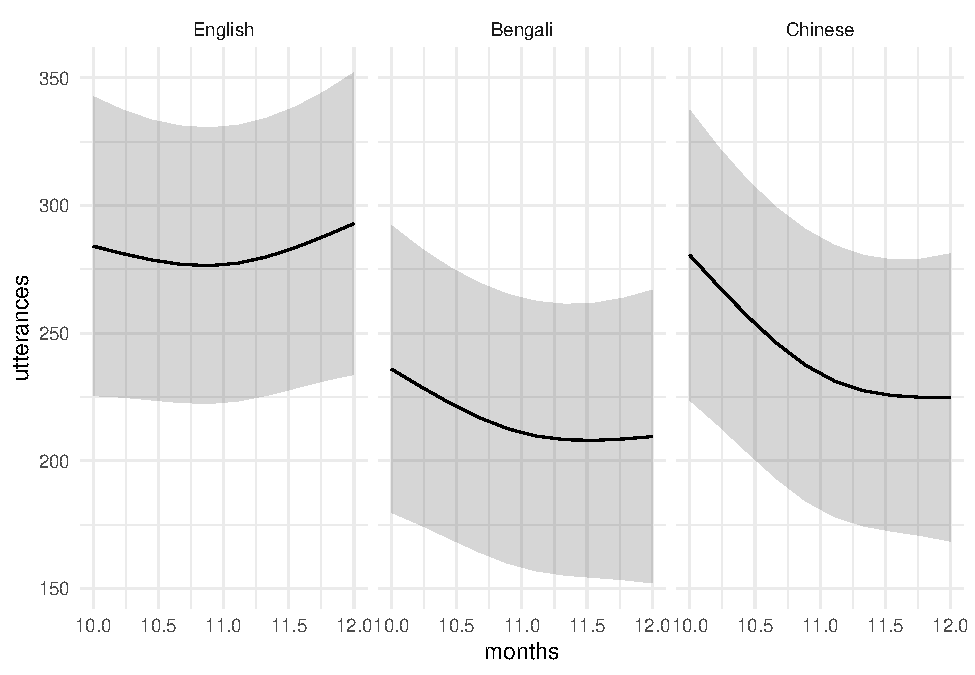
\includegraphics{supplement_files/figure-latex/utter-gam-plot-1.pdf}

\begin{center}\rule{0.5\linewidth}{\linethickness}\end{center}

The following models test time sample.

\begin{Shaded}
\begin{Highlighting}[]
\NormalTok{utter_gam_}\DecValTok{2}\NormalTok{ <-}\StringTok{ }\KeywordTok{gam}\NormalTok{(}
\NormalTok{  utterances }\OperatorTok{~}
\StringTok{    }\KeywordTok{s}\NormalTok{(months, }\DataTypeTok{k =} \DecValTok{3}\NormalTok{) }\OperatorTok{+}
\StringTok{    }\KeywordTok{s}\NormalTok{(months, dyad, }\DataTypeTok{k =} \DecValTok{2}\NormalTok{, }\DataTypeTok{bs =} \StringTok{"fs"}\NormalTok{, }\DataTypeTok{m =} \DecValTok{1}\NormalTok{),}
  \DataTypeTok{data =}\NormalTok{ utterances_tot,}
  \DataTypeTok{method =} \StringTok{"ML"}
\NormalTok{)}
\end{Highlighting}
\end{Shaded}

\begin{verbatim}
## Warning in gam.side(sm, X, tol = .Machine$double.eps^0.5): model has repeated 1-
## d smooths of same variable.
\end{verbatim}

\begin{Shaded}
\begin{Highlighting}[]
\NormalTok{utter_gam_}\DecValTok{2}\NormalTok{_null <-}\StringTok{ }\KeywordTok{gam}\NormalTok{(}
\NormalTok{  utterances }\OperatorTok{~}
\StringTok{    }\CommentTok{# s(months, k = 3) +}
\StringTok{    }\KeywordTok{s}\NormalTok{(months, dyad, }\DataTypeTok{k =} \DecValTok{2}\NormalTok{, }\DataTypeTok{bs =} \StringTok{"fs"}\NormalTok{, }\DataTypeTok{m =} \DecValTok{1}\NormalTok{),}
  \DataTypeTok{data =}\NormalTok{ utterances_tot,}
  \DataTypeTok{method =} \StringTok{"ML"}
\NormalTok{)}

\KeywordTok{compareML}\NormalTok{(utter_gam_}\DecValTok{2}\NormalTok{_null, utter_gam_}\DecValTok{2}\NormalTok{)}
\end{Highlighting}
\end{Shaded}

\begin{verbatim}
## utter_gam_2_null: utterances ~ s(months, dyad, k = 2, bs = "fs", m = 1)
## 
## utter_gam_2: utterances ~ s(months, k = 3) + s(months, dyad, k = 2, bs = "fs", 
##     m = 1)
## 
## Chi-square test of ML scores
## -----
##              Model    Score Edf Difference    Df p.value Sig.
## 1 utter_gam_2_null 1015.790   3                              
## 2      utter_gam_2 1013.245   5      2.545 2.000   0.078     
## 
## AIC difference: 6.82, model utter_gam_2 has lower AIC.
\end{verbatim}

\begin{verbatim}
## Warning in compareML(utter_gam_2_null, utter_gam_2): Only small difference in ML...
\end{verbatim}

\begin{Shaded}
\begin{Highlighting}[]
\KeywordTok{plot_smooths}\NormalTok{(utter_gam_}\DecValTok{2}\NormalTok{, months, }\DataTypeTok{series_length =} \DecValTok{10}\NormalTok{) }\OperatorTok{+}
\StringTok{  }\KeywordTok{labs}\NormalTok{(}\DataTypeTok{x =} \StringTok{"Months"}\NormalTok{, }\DataTypeTok{y =} \StringTok{"Count of utterances"}\NormalTok{, }\DataTypeTok{title =} \StringTok{"Predicted development of utterances"}\NormalTok{)}
\end{Highlighting}
\end{Shaded}

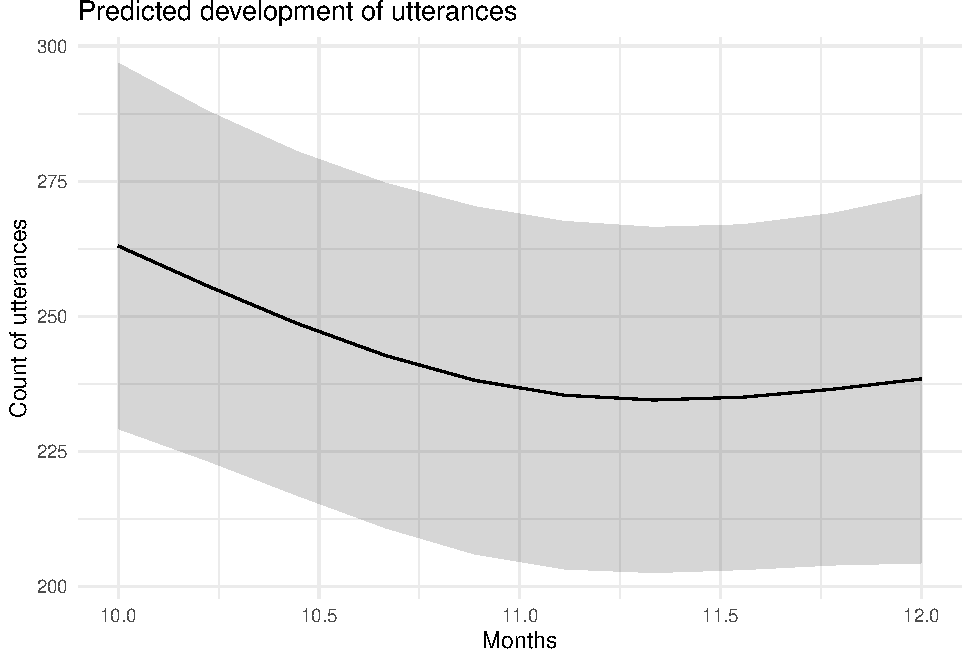
\includegraphics{supplement_files/figure-latex/utter-gam-2-plot-1.pdf}

\hypertarget{contingent-talks-development}{%
\subsection{Contingent talks
development}\label{contingent-talks-development}}

\begin{Shaded}
\begin{Highlighting}[]
\NormalTok{all_tot }\OperatorTok
\StringTok{  }\KeywordTok{ggplot}\NormalTok{(}\KeywordTok{aes}\NormalTok{(ct)) }\OperatorTok{+}\StringTok{ }\KeywordTok{geom_density}\NormalTok{() }\OperatorTok{+}\StringTok{ }\KeywordTok{geom_rug}\NormalTok{(}\DataTypeTok{alpha =} \FloatTok{0.1}\NormalTok{) }\OperatorTok{+}
\StringTok{  }\KeywordTok{labs}\NormalTok{(}
    \DataTypeTok{title =} \StringTok{"Distribution of the count of CTs"}\NormalTok{,}
    \DataTypeTok{x =} \StringTok{"Count of maternal CTs"}
\NormalTok{  )}
\end{Highlighting}
\end{Shaded}

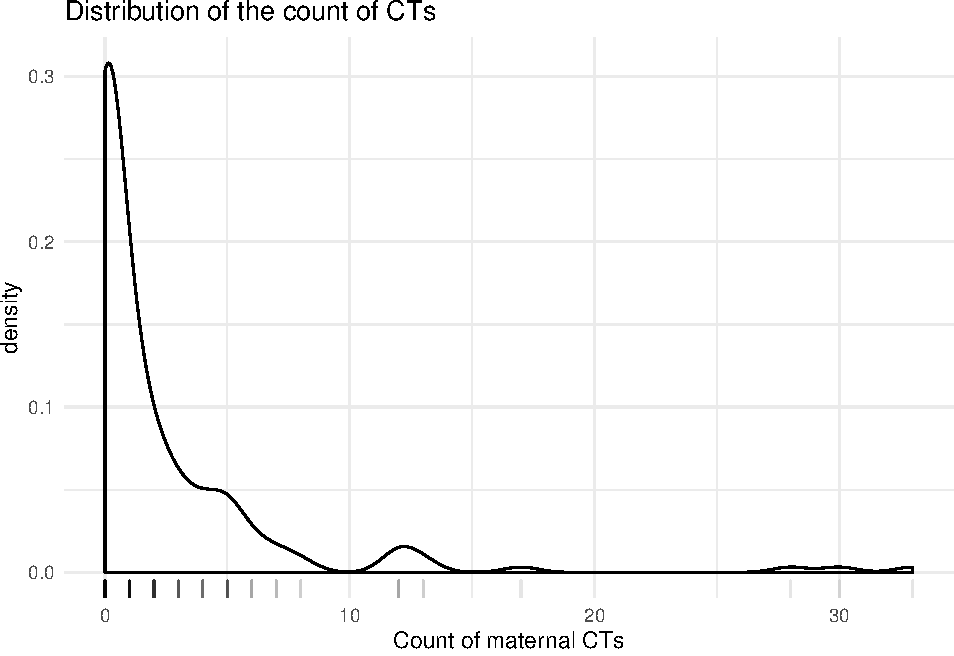
\includegraphics{supplement_files/figure-latex/ct-1.pdf}

\begin{center}\rule{0.5\linewidth}{\linethickness}\end{center}

The following models test cultural group.

\begin{Shaded}
\begin{Highlighting}[]
\NormalTok{ct_nb <-}\StringTok{ }\KeywordTok{glm.nb}\NormalTok{(ct }\OperatorTok{~}\StringTok{ }\NormalTok{months, }\DataTypeTok{data =}\NormalTok{ all_tot)}
\NormalTok{theta_}\DecValTok{4}\NormalTok{ <-}\StringTok{ }\KeywordTok{summary}\NormalTok{(ct_nb)[[}\StringTok{"theta"}\NormalTok{]]}

\NormalTok{ct_gam <-}\StringTok{ }\KeywordTok{gam}\NormalTok{(}
\NormalTok{  ct }\OperatorTok{~}
\StringTok{    }\NormalTok{back_o }\OperatorTok{+}
\StringTok{    }\KeywordTok{s}\NormalTok{(months, }\DataTypeTok{k =} \DecValTok{3}\NormalTok{) }\OperatorTok{+}
\StringTok{    }\KeywordTok{s}\NormalTok{(months, }\DataTypeTok{k =} \DecValTok{3}\NormalTok{, }\DataTypeTok{by =}\NormalTok{ back_o) }\OperatorTok{+}
\StringTok{    }\KeywordTok{s}\NormalTok{(months, dyad, }\DataTypeTok{k =} \DecValTok{2}\NormalTok{, }\DataTypeTok{bs =} \StringTok{"fs"}\NormalTok{, }\DataTypeTok{m =} \DecValTok{1}\NormalTok{),}
  \DataTypeTok{data =}\NormalTok{ all_tot,}
  \DataTypeTok{method =} \StringTok{"ML"}\NormalTok{,}
  \DataTypeTok{family =} \KeywordTok{negbin}\NormalTok{(theta_}\DecValTok{4}\NormalTok{)}
\NormalTok{)}
\end{Highlighting}
\end{Shaded}

\begin{verbatim}
## Warning in gam.side(sm, X, tol = .Machine$double.eps^0.5): model has repeated 1-
## d smooths of same variable.
\end{verbatim}

\begin{Shaded}
\begin{Highlighting}[]
\KeywordTok{summary}\NormalTok{(ct_gam)}
\end{Highlighting}
\end{Shaded}

\begin{verbatim}
## 
## Family: Negative Binomial(0.373) 
## Link function: log 
## 
## Formula:
## ct ~ back_o + s(months, k = 3) + s(months, k = 3, by = back_o) + 
##     s(months, dyad, k = 2, bs = "fs", m = 1)
## 
## Parametric coefficients:
##               Estimate Std. Error z value Pr(>|z|)  
## (Intercept)     0.5592     0.2975   1.879   0.0602 .
## back_oBengali  -0.9037     0.4387  -2.060   0.0394 *
## back_oChinese  -0.1228     0.4266  -0.288   0.7735  
## ---
## Signif. codes:  0 '***' 0.001 '**' 0.01 '*' 0.05 '.' 0.1 ' ' 1
## 
## Approximate significance of smooth terms:
##                            edf  Ref.df Chi.sq p-value   
## s(months)                1.000   1.000  3.079 0.07930 . 
## s(months):back_oBengali  1.746   1.935  3.004 0.24773   
## s(months):back_oChinese  1.000   1.000  0.388 0.53359   
## s(months,dyad)          19.141 114.000 28.993 0.00767 **
## ---
## Signif. codes:  0 '***' 0.001 '**' 0.01 '*' 0.05 '.' 0.1 ' ' 1
## 
## R-sq.(adj) =  0.392   Deviance explained =   44%
## -ML =    318  Scale est. = 1         n = 175
\end{verbatim}

\begin{Shaded}
\begin{Highlighting}[]
\NormalTok{ct_gam_null <-}\StringTok{ }\KeywordTok{gam}\NormalTok{(}
\NormalTok{  ct }\OperatorTok{~}
\StringTok{    }\CommentTok{# back_o +}
\StringTok{    }\KeywordTok{s}\NormalTok{(months, }\DataTypeTok{k =} \DecValTok{3}\NormalTok{) }\OperatorTok{+}
\StringTok{    }\CommentTok{# s(months, k = 3, by = back_o) +}
\StringTok{    }\KeywordTok{s}\NormalTok{(months, dyad, }\DataTypeTok{k =} \DecValTok{2}\NormalTok{, }\DataTypeTok{bs =} \StringTok{"fs"}\NormalTok{, }\DataTypeTok{m =} \DecValTok{1}\NormalTok{),}
  \DataTypeTok{data =}\NormalTok{ all_tot,}
  \DataTypeTok{method =} \StringTok{"ML"}\NormalTok{,}
  \DataTypeTok{family =} \KeywordTok{negbin}\NormalTok{(theta_}\DecValTok{4}\NormalTok{)}
\NormalTok{)}
\end{Highlighting}
\end{Shaded}

\begin{verbatim}
## Warning in gam.side(sm, X, tol = .Machine$double.eps^0.5): model has repeated 1-
## d smooths of same variable.
\end{verbatim}

\begin{Shaded}
\begin{Highlighting}[]
\KeywordTok{compareML}\NormalTok{(ct_gam_null, ct_gam)}
\end{Highlighting}
\end{Shaded}

\begin{verbatim}
## ct_gam_null: ct ~ s(months, k = 3) + s(months, dyad, k = 2, bs = "fs", m = 1)
## 
## ct_gam: ct ~ back_o + s(months, k = 3) + s(months, k = 3, by = back_o) + 
##     s(months, dyad, k = 2, bs = "fs", m = 1)
## 
## Chi-square test of ML scores
## -----
##         Model    Score Edf Difference    Df p.value Sig.
## 1 ct_gam_null 321.0879   5                              
## 2      ct_gam 318.0012  11      3.087 6.000   0.404     
## 
## AIC difference: 0.14, model ct_gam has lower AIC.
\end{verbatim}

\begin{verbatim}
## Warning in compareML(ct_gam_null, ct_gam): Only small difference in ML...
\end{verbatim}

\begin{Shaded}
\begin{Highlighting}[]
\KeywordTok{plot_smooths}\NormalTok{(ct_gam, months, }\DataTypeTok{facet_terms =}\NormalTok{ back_o, }\DataTypeTok{series_length =} \DecValTok{10}\NormalTok{, }\DataTypeTok{transform =}\NormalTok{ exp) }\OperatorTok{+}
\StringTok{  }\KeywordTok{labs}\NormalTok{(}\DataTypeTok{x =} \StringTok{"Months"}\NormalTok{, }\DataTypeTok{y =} \StringTok{"Count of CTs"}\NormalTok{, }\DataTypeTok{title =} \StringTok{"Predicted development of CTs by background"}\NormalTok{)}
\end{Highlighting}
\end{Shaded}

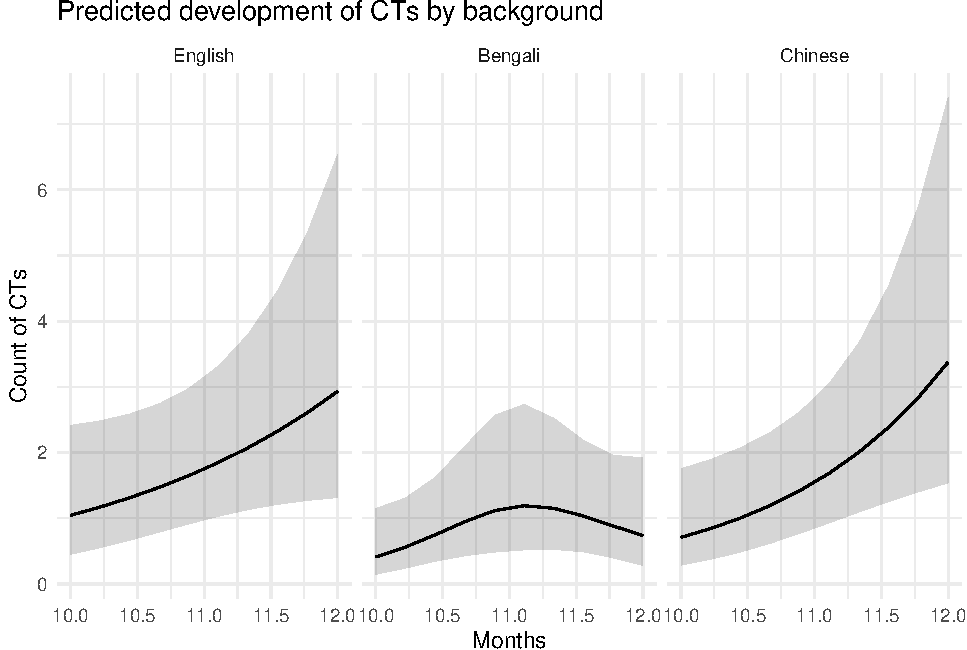
\includegraphics{supplement_files/figure-latex/ct-gam-plot-1.pdf}

\begin{center}\rule{0.5\linewidth}{\linethickness}\end{center}

The following models test time sample.

\begin{Shaded}
\begin{Highlighting}[]
\NormalTok{ct_gam_}\DecValTok{2}\NormalTok{ <-}\StringTok{ }\KeywordTok{gam}\NormalTok{(}
\NormalTok{  count }\OperatorTok{~}
\StringTok{    }\KeywordTok{s}\NormalTok{(months, }\DataTypeTok{k =} \DecValTok{3}\NormalTok{) }\OperatorTok{+}
\StringTok{    }\KeywordTok{s}\NormalTok{(months, dyad, }\DataTypeTok{k =} \DecValTok{2}\NormalTok{, }\DataTypeTok{bs =} \StringTok{"fs"}\NormalTok{, }\DataTypeTok{m =} \DecValTok{1}\NormalTok{),}
  \DataTypeTok{data =}\NormalTok{ all_tot,}
  \DataTypeTok{method =} \StringTok{"ML"}\NormalTok{,}
  \DataTypeTok{family =} \KeywordTok{negbin}\NormalTok{(theta_}\DecValTok{4}\NormalTok{)}
\NormalTok{)}
\end{Highlighting}
\end{Shaded}

\begin{verbatim}
## Warning in gam.side(sm, X, tol = .Machine$double.eps^0.5): model has repeated 1-
## d smooths of same variable.
\end{verbatim}

\begin{Shaded}
\begin{Highlighting}[]
\NormalTok{ct_gam_}\DecValTok{2}\NormalTok{_null <-}\StringTok{ }\KeywordTok{gam}\NormalTok{(}
\NormalTok{  count }\OperatorTok{~}
\StringTok{    }\CommentTok{# s(months, k = 3) +}
\StringTok{    }\KeywordTok{s}\NormalTok{(months, dyad, }\DataTypeTok{k =} \DecValTok{2}\NormalTok{, }\DataTypeTok{bs =} \StringTok{"fs"}\NormalTok{, }\DataTypeTok{m =} \DecValTok{1}\NormalTok{),}
  \DataTypeTok{data =}\NormalTok{ all_tot,}
  \DataTypeTok{method =} \StringTok{"ML"}\NormalTok{,}
  \DataTypeTok{family =} \KeywordTok{negbin}\NormalTok{(theta_}\DecValTok{4}\NormalTok{)}
\NormalTok{)}

\KeywordTok{compareML}\NormalTok{(ct_gam_}\DecValTok{2}\NormalTok{_null, ct_gam_}\DecValTok{2}\NormalTok{)}
\end{Highlighting}
\end{Shaded}

\begin{verbatim}
## ct_gam_2_null: count ~ s(months, dyad, k = 2, bs = "fs", m = 1)
## 
## ct_gam_2: count ~ s(months, k = 3) + s(months, dyad, k = 2, bs = "fs", 
##     m = 1)
## 
## Chi-square test of ML scores
## -----
##           Model    Score Edf Difference    Df p.value Sig.
## 1 ct_gam_2_null 649.9766   3                              
## 2      ct_gam_2 645.5516   5      4.425 2.000   0.012  *  
## 
## AIC difference: 6.85, model ct_gam_2 has lower AIC.
\end{verbatim}

\begin{verbatim}
## Warning in compareML(ct_gam_2_null, ct_gam_2): Only small difference in ML...
\end{verbatim}

\begin{Shaded}
\begin{Highlighting}[]
\KeywordTok{plot_smooths}\NormalTok{(ct_gam_}\DecValTok{2}\NormalTok{, months, }\DataTypeTok{series_length =} \DecValTok{10}\NormalTok{, }\DataTypeTok{transform =}\NormalTok{ exp) }\OperatorTok{+}
\StringTok{  }\KeywordTok{labs}\NormalTok{(}\DataTypeTok{x =} \StringTok{"Months"}\NormalTok{, }\DataTypeTok{y =} \StringTok{"Count of CTs"}\NormalTok{, }\DataTypeTok{title =} \StringTok{"Predicted development of CTs"}\NormalTok{)}
\end{Highlighting}
\end{Shaded}

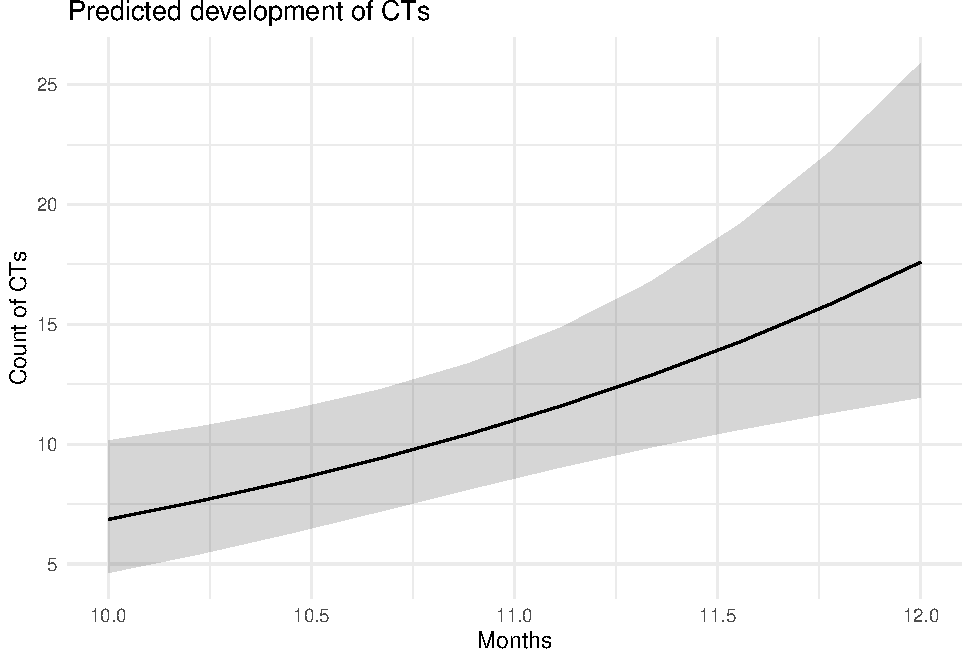
\includegraphics{supplement_files/figure-latex/ct-gam-2-plot-1.pdf}

\newpage

\hypertarget{analysis-1c.-predictors-of-pointing}{%
\section{Analysis 1c. Predictors of
pointing}\label{analysis-1c.-predictors-of-pointing}}

The following GLMMs test the relation between pointing and reaches/HoGs.
The count of pointing refers to the one produced by the infant in the
subsequent session: For example, the count of reaches at 10 months is
matched with the count of points at 11 months, and that of reaches at 11
months is matched with the count of points at 12 months. This allows us
to test whether gestures at a certain sampling time predict the
production of pointing at the next sampling time. Data on pointing at 10
months is dropped, since there is no data on gestures prior to 10
months.

\hypertarget{reaches}{%
\subsection{Reaches}\label{reaches}}

\begin{Shaded}
\begin{Highlighting}[]
\NormalTok{reach_point_lead_nb <-}\StringTok{ }\KeywordTok{glm.nb}\NormalTok{(lead_point }\OperatorTok{~}\StringTok{ }\NormalTok{reach, }\DataTypeTok{data =}\NormalTok{ reach_point_lead)}
\NormalTok{theta_}\DecValTok{5}\NormalTok{ <-}\StringTok{ }\KeywordTok{summary}\NormalTok{(reach_point_lead_nb)[[}\StringTok{"theta"}\NormalTok{]]}

\NormalTok{reach_point_lm <-}\StringTok{ }\KeywordTok{glmer}\NormalTok{(}
\NormalTok{  lead_point }\OperatorTok{~}
\StringTok{    }\NormalTok{reach }\OperatorTok{*}
\StringTok{    }\NormalTok{background }\OperatorTok{+}
\StringTok{    }\NormalTok{(}\DecValTok{1}\OperatorTok{|}\NormalTok{dyad),}
  \DataTypeTok{data =}\NormalTok{ reach_point_lead,}
  \DataTypeTok{family =} \KeywordTok{negbin}\NormalTok{(theta_}\DecValTok{5}\NormalTok{)}
\NormalTok{)}
\end{Highlighting}
\end{Shaded}

\begin{verbatim}
## Warning in checkConv(attr(opt, "derivs"), opt$par, ctrl = control$checkConv, :
## unable to evaluate scaled gradient
\end{verbatim}

\begin{verbatim}
## Warning in checkConv(attr(opt, "derivs"), opt$par, ctrl = control$checkConv, :
## Model failed to converge: degenerate Hessian with 1 negative eigenvalues
\end{verbatim}

\begin{Shaded}
\begin{Highlighting}[]
\KeywordTok{summary}\NormalTok{(reach_point_lm)}
\end{Highlighting}
\end{Shaded}

\begin{verbatim}
## Warning in vcov.merMod(object, use.hessian = use.hessian): variance-covariance matrix computed from finite-difference Hessian is
## not positive definite or contains NA values: falling back to var-cov estimated from RX
\end{verbatim}

\begin{verbatim}
## Warning in vcov.merMod(object, correlation = correlation, sigm = sig): variance-covariance matrix computed from finite-difference Hessian is
## not positive definite or contains NA values: falling back to var-cov estimated from RX
\end{verbatim}

\begin{verbatim}
## Generalized linear mixed model fit by maximum likelihood (Laplace
##   Approximation) [glmerMod]
##  Family: Negative Binomial(0.26)  ( log )
## Formula: lead_point ~ reach * background + (1 | dyad)
##    Data: reach_point_lead
## 
##      AIC      BIC   logLik deviance df.resid 
##    526.7    548.5   -255.3    510.7      106 
## 
## Scaled residuals: 
##     Min      1Q  Median      3Q     Max 
## -0.4989 -0.4914 -0.3940  0.1764  3.0988 
## 
## Random effects:
##  Groups Name        Variance Std.Dev.
##  dyad   (Intercept) 0.1822   0.4269  
## Number of obs: 114, groups:  dyad, 58
## 
## Fixed effects:
##                         Estimate Std. Error z value Pr(>|z|)
## (Intercept)              0.70291    0.52375   1.342    0.180
## reach                    0.06262    0.09957   0.629    0.529
## backgroundChinese        1.11638    0.71143   1.569    0.117
## backgroundEnglish        0.74792    0.66268   1.129    0.259
## reach:backgroundChinese -0.24857    0.15914  -1.562    0.118
## reach:backgroundEnglish -0.07719    0.15523  -0.497    0.619
## 
## Correlation of Fixed Effects:
##             (Intr) reach  bckgrC bckgrE rch:bC
## reach       -0.747                            
## bckgrndChns -0.736  0.550                     
## bckgrndEngl -0.790  0.590  0.582              
## rch:bckgrnC  0.467 -0.626 -0.707 -0.369       
## rch:bckgrnE  0.479 -0.641 -0.353 -0.639  0.401
## convergence code: 0
## unable to evaluate scaled gradient
## Model failed to converge: degenerate  Hessian with 1 negative eigenvalues
\end{verbatim}

\begin{Shaded}
\begin{Highlighting}[]
\KeywordTok{plot_model}\NormalTok{(reach_point_lm, }\DataTypeTok{type =} \StringTok{"pred"}\NormalTok{, }\DataTypeTok{terms =} \KeywordTok{c}\NormalTok{(}\StringTok{"reach"}\NormalTok{, }\StringTok{"background"}\NormalTok{))}
\end{Highlighting}
\end{Shaded}

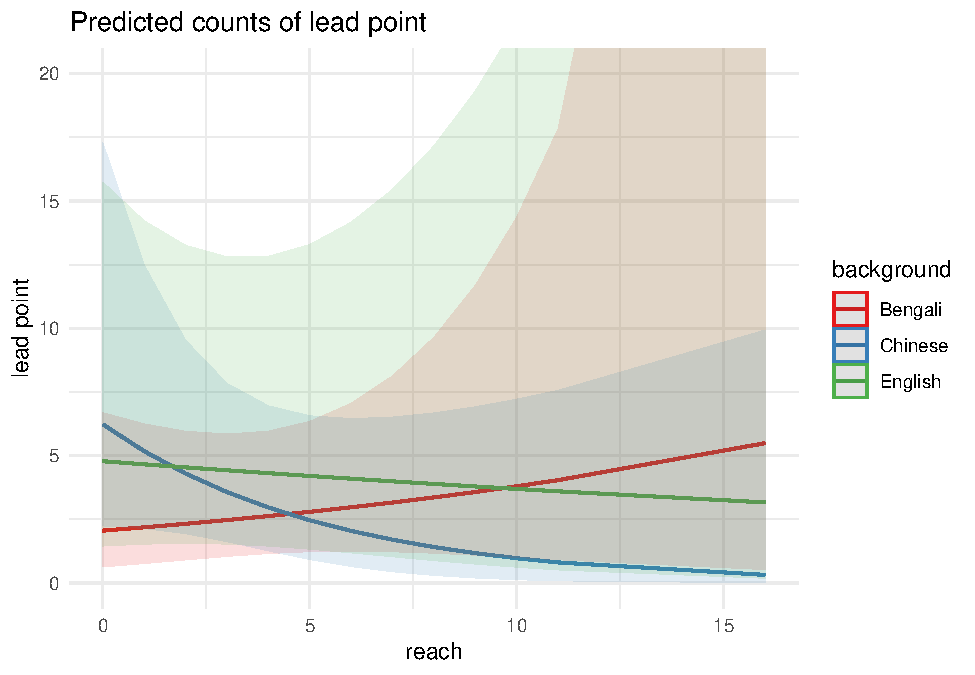
\includegraphics{supplement_files/figure-latex/reach-point-plot-1.pdf}

\hypertarget{hogs}{%
\subsection{HoGs}\label{hogs}}

\begin{Shaded}
\begin{Highlighting}[]
\NormalTok{hg_point_lead_nb <-}\StringTok{ }\KeywordTok{glm.nb}\NormalTok{(lead_point }\OperatorTok{~}\StringTok{ }\NormalTok{ho_gv, }\DataTypeTok{data =} \KeywordTok{filter}\NormalTok{(hg_point_lead, ho_gv }\OperatorTok{<}\StringTok{ }\DecValTok{20}\NormalTok{))}
\NormalTok{theta_}\DecValTok{6}\NormalTok{ <-}\StringTok{ }\KeywordTok{summary}\NormalTok{(reach_point_lead_nb)[[}\StringTok{"theta"}\NormalTok{]]}

\NormalTok{hg_point_lm <-}\StringTok{ }\KeywordTok{glmer}\NormalTok{(}
\NormalTok{  lead_point }\OperatorTok{~}
\StringTok{    }\NormalTok{ho_gv }\OperatorTok{*}
\StringTok{    }\NormalTok{background }\OperatorTok{+}
\StringTok{    }\NormalTok{(}\DecValTok{1}\OperatorTok{|}\NormalTok{dyad),}
  \DataTypeTok{data =} \KeywordTok{filter}\NormalTok{(hg_point_lead, ho_gv }\OperatorTok{<}\StringTok{ }\DecValTok{20}\NormalTok{),}
  \DataTypeTok{family =} \KeywordTok{negbin}\NormalTok{(theta_}\DecValTok{6}\NormalTok{)}
\NormalTok{)}
\KeywordTok{summary}\NormalTok{(hg_point_lm)}
\end{Highlighting}
\end{Shaded}

\begin{verbatim}
## Generalized linear mixed model fit by maximum likelihood (Laplace
##   Approximation) [glmerMod]
##  Family: Negative Binomial(0.26)  ( log )
## Formula: lead_point ~ ho_gv * background + (1 | dyad)
##    Data: filter(hg_point_lead, ho_gv < 20)
## 
##      AIC      BIC   logLik deviance df.resid 
##    506.6    528.2   -245.3    490.6      103 
## 
## Scaled residuals: 
##     Min      1Q  Median      3Q     Max 
## -0.5073 -0.4924 -0.4106  0.1212  6.4456 
## 
## Random effects:
##  Groups Name        Variance Std.Dev.
##  dyad   (Intercept) 0.005369 0.07328 
## Number of obs: 111, groups:  dyad, 58
## 
## Fixed effects:
##                         Estimate Std. Error z value Pr(>|z|)   
## (Intercept)              1.37213    0.48622   2.822  0.00477 **
## ho_gv                   -0.10704    0.08076  -1.325  0.18503   
## backgroundChinese        0.11309    0.69265   0.163  0.87030   
## backgroundEnglish       -0.30788    0.66637  -0.462  0.64406   
## ho_gv:backgroundChinese  0.12669    0.13919   0.910  0.36274   
## ho_gv:backgroundEnglish  0.33116    0.15724   2.106  0.03520 * 
## ---
## Signif. codes:  0 '***' 0.001 '**' 0.01 '*' 0.05 '.' 0.1 ' ' 1
## 
## Correlation of Fixed Effects:
##             (Intr) ho_gv  bckgrC bckgrE h_gv:C
## ho_gv       -0.672                            
## bckgrndChns -0.627  0.452                     
## bckgrndEngl -0.569  0.449  0.490              
## h_gv:bckgrC  0.388 -0.580 -0.710 -0.263       
## h_gv:bckgrE  0.350 -0.515 -0.231 -0.556  0.298
\end{verbatim}

\begin{Shaded}
\begin{Highlighting}[]
\KeywordTok{plot_model}\NormalTok{(hg_point_lm, }\DataTypeTok{type =} \StringTok{"pred"}\NormalTok{, }\DataTypeTok{terms =} \KeywordTok{c}\NormalTok{(}\StringTok{"ho_gv"}\NormalTok{, }\StringTok{"background"}\NormalTok{))}
\end{Highlighting}
\end{Shaded}

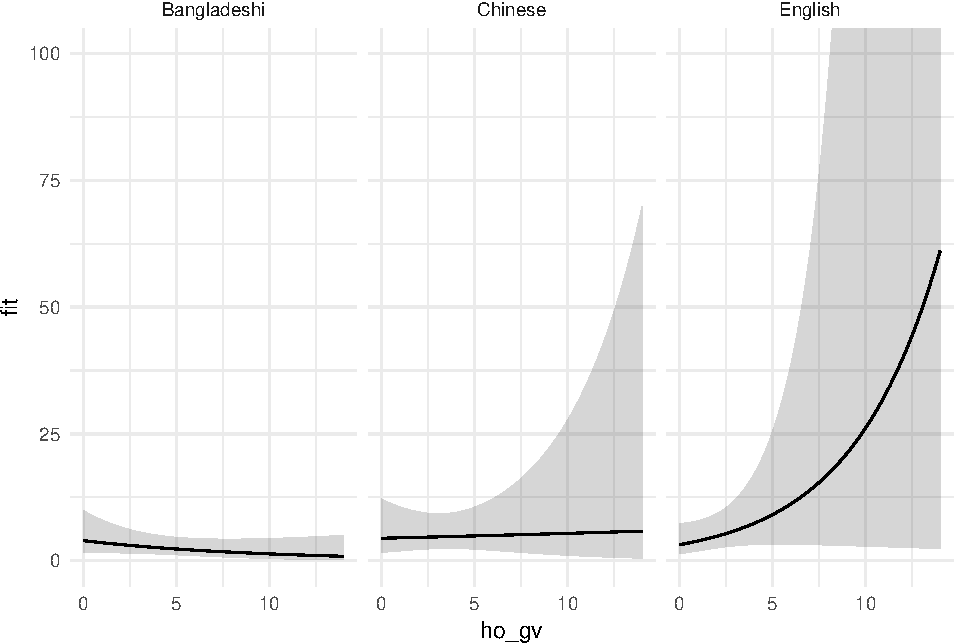
\includegraphics{supplement_files/figure-latex/hg-point-plot-1.pdf}

\newpage

\hypertarget{analysis-2.-predictors-of-vocabulary-scores-at-12-and-18-months}{%
\section{Analysis 2. Predictors of vocabulary scores at 12 and 18
months}\label{analysis-2.-predictors-of-vocabulary-scores-at-12-and-18-months}}

\hypertarget{comprehension-at-12-and-18-months}{%
\subsection{Comprehension at 12 and 18
months}\label{comprehension-at-12-and-18-months}}

\hypertarget{all-gestures-combined}{%
\subsubsection{All gestures combined}\label{all-gestures-combined}}

\begin{Shaded}
\begin{Highlighting}[]
\NormalTok{all_gest_lm <-}\StringTok{ }\KeywordTok{glm}\NormalTok{(}
\NormalTok{  comprehension }\OperatorTok{~}
\StringTok{    }\NormalTok{count_tot }\OperatorTok{*}
\StringTok{    }\NormalTok{months }\OperatorTok{*}
\StringTok{    }\NormalTok{background,}
  \DataTypeTok{data =}\NormalTok{ vocab}
\NormalTok{)}
\KeywordTok{summary}\NormalTok{(all_gest_lm)}
\end{Highlighting}
\end{Shaded}

\begin{verbatim}
## 
## Call:
## glm(formula = comprehension ~ count_tot * months * background, 
##     data = vocab)
## 
## Deviance Residuals: 
##     Min       1Q   Median       3Q      Max  
## -156.70   -39.73    -5.75    35.51   171.23  
## 
## Coefficients:
##                                        Estimate Std. Error t value Pr(>|t|)    
## (Intercept)                          104.819001  21.015944   4.988 2.61e-06 ***
## count_tot                             -0.378321   0.430875  -0.878 0.382054    
## months18                             110.696502  30.293421   3.654 0.000415 ***
## backgroundBengali                      7.278570  41.339385   0.176 0.860600    
## backgroundChinese                    -89.225349  35.938992  -2.483 0.014721 *  
## count_tot:months18                     0.699017   0.612716   1.141 0.256685    
## count_tot:backgroundBengali            0.067434   0.910717   0.074 0.941124    
## count_tot:backgroundChinese            2.535049   0.733392   3.457 0.000807 ***
## months18:backgroundBengali           -48.881085  58.755775  -0.832 0.407447    
## months18:backgroundChinese            10.532049  51.162231   0.206 0.837326    
## count_tot:months18:backgroundBengali   0.005265   1.289544   0.004 0.996751    
## count_tot:months18:backgroundChinese  -0.653531   1.039154  -0.629 0.530858    
## ---
## Signif. codes:  0 '***' 0.001 '**' 0.01 '*' 0.05 '.' 0.1 ' ' 1
## 
## (Dispersion parameter for gaussian family taken to be 5070.59)
## 
##     Null deviance: 1029475  on 110  degrees of freedom
## Residual deviance:  501988  on  99  degrees of freedom
##   (9 observations deleted due to missingness)
## AIC: 1275.3
## 
## Number of Fisher Scoring iterations: 2
\end{verbatim}

\begin{Shaded}
\begin{Highlighting}[]
\KeywordTok{plot_model}\NormalTok{(all_gest_lm, }\DataTypeTok{type =} \StringTok{"pred"}\NormalTok{, }\DataTypeTok{terms =} \KeywordTok{c}\NormalTok{(}\StringTok{"count_tot"}\NormalTok{, }\StringTok{"months"}\NormalTok{, }\StringTok{"background"}\NormalTok{))}
\end{Highlighting}
\end{Shaded}

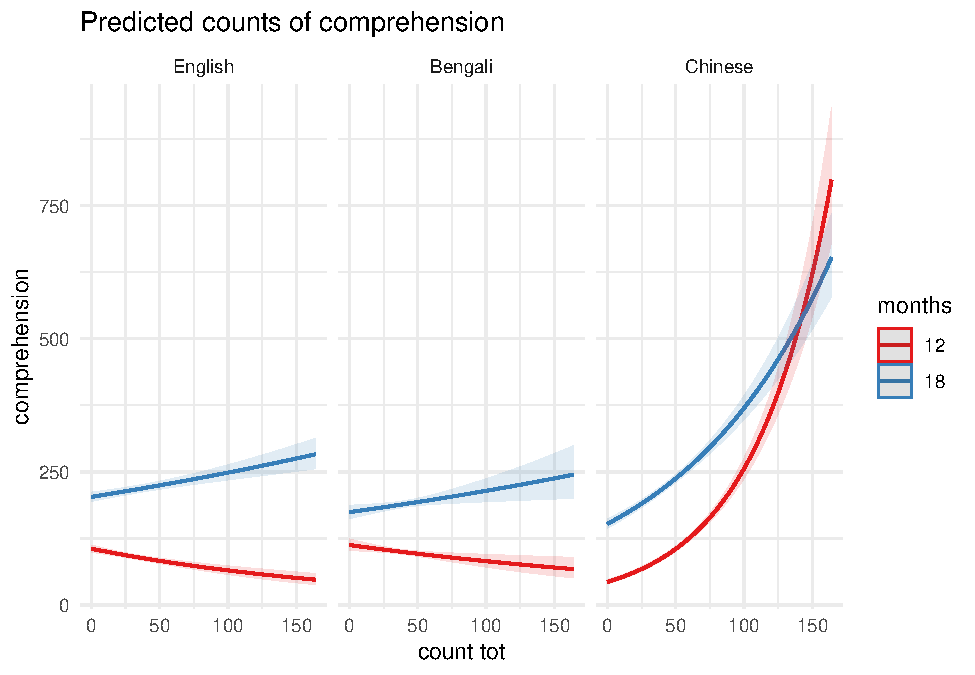
\includegraphics{supplement_files/figure-latex/all-gest-lm-plot-1.pdf}

\hypertarget{hogs-points}{%
\subsubsection{HoGs + points}\label{hogs-points}}

\begin{Shaded}
\begin{Highlighting}[]
\NormalTok{hgp_lm <-}\StringTok{ }\KeywordTok{glm}\NormalTok{(}
\NormalTok{  comprehension }\OperatorTok{~}
\StringTok{    }\NormalTok{hgp_tot }\OperatorTok{*}
\StringTok{    }\NormalTok{months }\OperatorTok{*}
\StringTok{    }\NormalTok{background,}
  \DataTypeTok{data =}\NormalTok{ vocab}
\NormalTok{)}
\KeywordTok{summary}\NormalTok{(hgp_lm)}
\end{Highlighting}
\end{Shaded}

\begin{verbatim}
## 
## Call:
## glm(formula = comprehension ~ hgp_tot * months * background, 
##     data = vocab)
## 
## Deviance Residuals: 
##      Min        1Q    Median        3Q       Max  
## -151.270   -45.462    -3.292    40.113   190.745  
## 
## Coefficients:
##                                     Estimate Std. Error t value Pr(>|t|)    
## (Intercept)                        102.72656   19.74120   5.204 1.06e-06 ***
## hgp_tot                             -0.39563    0.43952  -0.900 0.370221    
## months18                           114.95177   28.45501   4.040 0.000106 ***
## backgroundBengali                    0.56846   37.26005   0.015 0.987858    
## backgroundChinese                  -63.18223   32.50198  -1.944 0.054740 .  
## hgp_tot:months18                     0.71535    0.62482   1.145 0.255014    
## hgp_tot:backgroundBengali            0.27301    1.04980   0.260 0.795360    
## hgp_tot:backgroundChinese            2.37494    0.75193   3.158 0.002103 ** 
## months18:backgroundBengali         -48.17944   52.97999  -0.909 0.365353    
## months18:backgroundChinese           6.13002   46.29271   0.132 0.894922    
## hgp_tot:months18:backgroundBengali   0.09461    1.48600   0.064 0.949366    
## hgp_tot:months18:backgroundChinese  -0.65302    1.06530  -0.613 0.541287    
## ---
## Signif. codes:  0 '***' 0.001 '**' 0.01 '*' 0.05 '.' 0.1 ' ' 1
## 
## (Dispersion parameter for gaussian family taken to be 5281.199)
## 
##     Null deviance: 1029475  on 110  degrees of freedom
## Residual deviance:  522839  on  99  degrees of freedom
##   (9 observations deleted due to missingness)
## AIC: 1279.8
## 
## Number of Fisher Scoring iterations: 2
\end{verbatim}

\begin{Shaded}
\begin{Highlighting}[]
\KeywordTok{plot_model}\NormalTok{(hgp_lm, }\DataTypeTok{type =} \StringTok{"pred"}\NormalTok{, }\DataTypeTok{terms =} \KeywordTok{c}\NormalTok{(}\StringTok{"hgp_tot"}\NormalTok{, }\StringTok{"months"}\NormalTok{, }\StringTok{"background"}\NormalTok{))}
\end{Highlighting}
\end{Shaded}

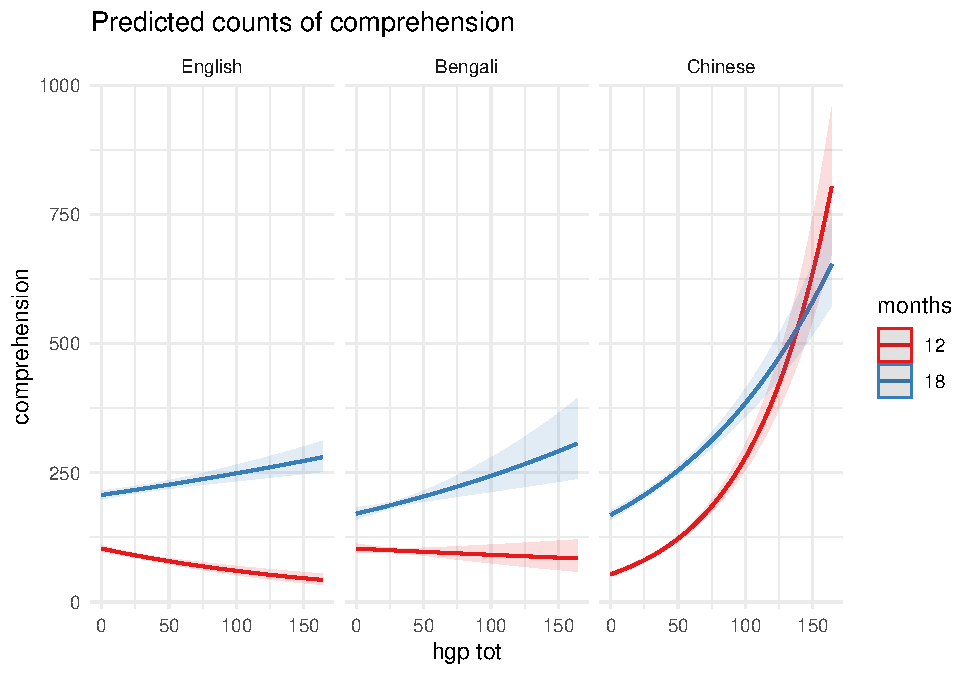
\includegraphics{supplement_files/figure-latex/hgp-lm-2-plot-1.pdf}

\hypertarget{reaches-1}{%
\subsubsection{Reaches}\label{reaches-1}}

\begin{Shaded}
\begin{Highlighting}[]
\NormalTok{reach_lm <-}\StringTok{ }\KeywordTok{glm}\NormalTok{(}
\NormalTok{  comprehension }\OperatorTok{~}
\StringTok{    }\NormalTok{reach_tot }\OperatorTok{*}
\StringTok{    }\NormalTok{months }\OperatorTok{*}
\StringTok{    }\NormalTok{background,}
  \DataTypeTok{data =}\NormalTok{ vocab}
\NormalTok{)}
\KeywordTok{summary}\NormalTok{(reach_lm)}
\end{Highlighting}
\end{Shaded}

\begin{verbatim}
## 
## Call:
## glm(formula = comprehension ~ reach_tot * months * background, 
##     data = vocab)
## 
## Deviance Residuals: 
##      Min        1Q    Median        3Q       Max  
## -197.044   -57.157    -0.536    49.498   209.415  
## 
## Coefficients:
##                                      Estimate Std. Error t value Pr(>|t|)    
## (Intercept)                           89.3681    25.5484   3.498 0.000704 ***
## reach_tot                              0.5794     2.7251   0.213 0.832060    
## months18                             136.3484    36.4306   3.743 0.000306 ***
## backgroundBengali                     34.5661    44.1284   0.783 0.435316    
## backgroundChinese                    -31.9806    42.3424  -0.755 0.451872    
## reach_tot:months18                    -0.5702     3.8544  -0.148 0.882690    
## reach_tot:backgroundBengali           -2.7184     3.8808  -0.700 0.485264    
## reach_tot:backgroundChinese            4.6953     4.2944   1.093 0.276901    
## months18:backgroundBengali           -58.4408    62.5810  -0.934 0.352656    
## months18:backgroundChinese            -9.8248    60.0626  -0.164 0.870398    
## reach_tot:months18:backgroundBengali   1.6065     5.4886   0.293 0.770369    
## reach_tot:months18:backgroundChinese   0.1622     6.0736   0.027 0.978746    
## ---
## Signif. codes:  0 '***' 0.001 '**' 0.01 '*' 0.05 '.' 0.1 ' ' 1
## 
## (Dispersion parameter for gaussian family taken to be 6196.532)
## 
##     Null deviance: 1029475  on 110  degrees of freedom
## Residual deviance:  613457  on  99  degrees of freedom
##   (9 observations deleted due to missingness)
## AIC: 1297.5
## 
## Number of Fisher Scoring iterations: 2
\end{verbatim}

\begin{Shaded}
\begin{Highlighting}[]
\KeywordTok{plot_model}\NormalTok{(reach_lm, }\DataTypeTok{type =} \StringTok{"pred"}\NormalTok{, }\DataTypeTok{terms =} \KeywordTok{c}\NormalTok{(}\StringTok{"reach_tot"}\NormalTok{, }\StringTok{"months"}\NormalTok{, }\StringTok{"background"}\NormalTok{))}
\end{Highlighting}
\end{Shaded}

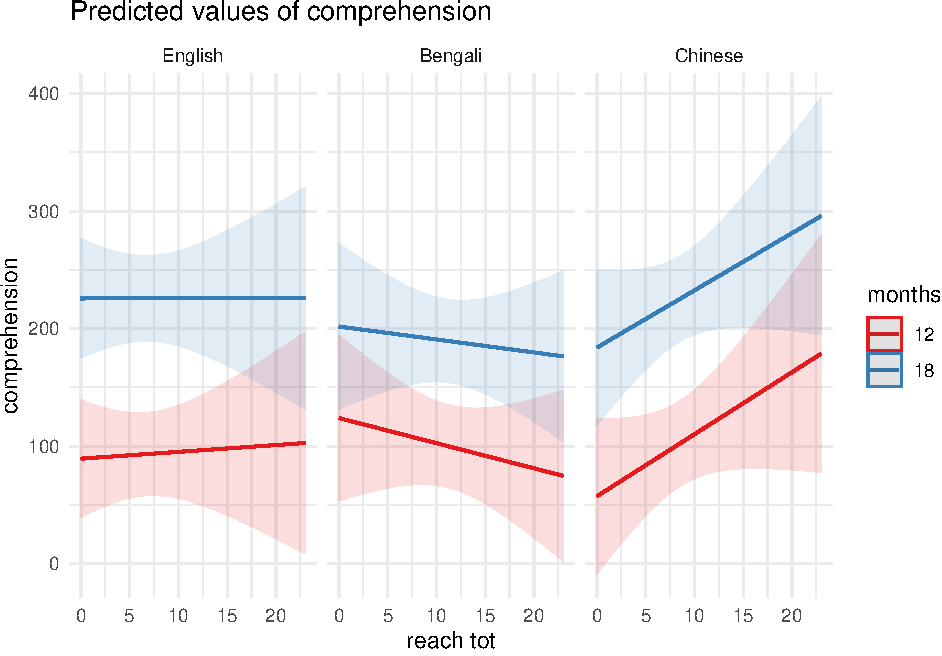
\includegraphics{supplement_files/figure-latex/reach-lm-2-plot-1.pdf}

\hypertarget{maternal-utterances}{%
\subsubsection{Maternal utterances}\label{maternal-utterances}}

\begin{Shaded}
\begin{Highlighting}[]
\NormalTok{utt_lm <-}\StringTok{ }\KeywordTok{glm}\NormalTok{(}
\NormalTok{  comprehension }\OperatorTok{~}
\StringTok{    }\NormalTok{utt_tot }\OperatorTok{*}
\StringTok{    }\NormalTok{months }\OperatorTok{*}
\StringTok{    }\NormalTok{background,}
  \DataTypeTok{data =}\NormalTok{ vocab}
\NormalTok{)}
\KeywordTok{summary}\NormalTok{(utt_lm)}
\end{Highlighting}
\end{Shaded}

\begin{verbatim}
## 
## Call:
## glm(formula = comprehension ~ utt_tot * months * background, 
##     data = vocab)
## 
## Deviance Residuals: 
##     Min       1Q   Median       3Q      Max  
## -173.66   -49.34   -14.18    44.09   203.25  
## 
## Coefficients:
##                                      Estimate Std. Error t value Pr(>|t|)   
## (Intercept)                         190.06494   67.93748   2.798  0.00631 **
## utt_tot                              -0.10670    0.08073  -1.322  0.18968   
## months18                            171.12877   97.44509   1.756  0.08250 . 
## backgroundBengali                  -101.55937   75.35016  -1.348  0.18113   
## backgroundChinese                  -136.00385   79.67120  -1.707  0.09130 . 
## utt_tot:months18                     -0.06703    0.11490  -0.583  0.56110   
## utt_tot:backgroundBengali             0.13399    0.09159   1.463  0.14702   
## utt_tot:backgroundChinese             0.16751    0.09496   1.764  0.08118 . 
## months18:backgroundBengali          -84.50957  107.79535  -0.784  0.43513   
## months18:backgroundChinese          -48.28443  113.84000  -0.424  0.67249   
## utt_tot:months18:backgroundBengali    0.07726    0.13017   0.594  0.55435   
## utt_tot:months18:backgroundChinese    0.06563    0.13492   0.486  0.62787   
## ---
## Signif. codes:  0 '***' 0.001 '**' 0.01 '*' 0.05 '.' 0.1 ' ' 1
## 
## (Dispersion parameter for gaussian family taken to be 6228.136)
## 
##     Null deviance: 928782  on 100  degrees of freedom
## Residual deviance: 554304  on  89  degrees of freedom
##   (19 observations deleted due to missingness)
## AIC: 1182.3
## 
## Number of Fisher Scoring iterations: 2
\end{verbatim}

\begin{Shaded}
\begin{Highlighting}[]
\KeywordTok{plot_model}\NormalTok{(utt_lm, }\DataTypeTok{type =} \StringTok{"pred"}\NormalTok{, }\DataTypeTok{terms =} \KeywordTok{c}\NormalTok{(}\StringTok{"utt_tot"}\NormalTok{, }\StringTok{"months"}\NormalTok{, }\StringTok{"background"}\NormalTok{))}
\end{Highlighting}
\end{Shaded}

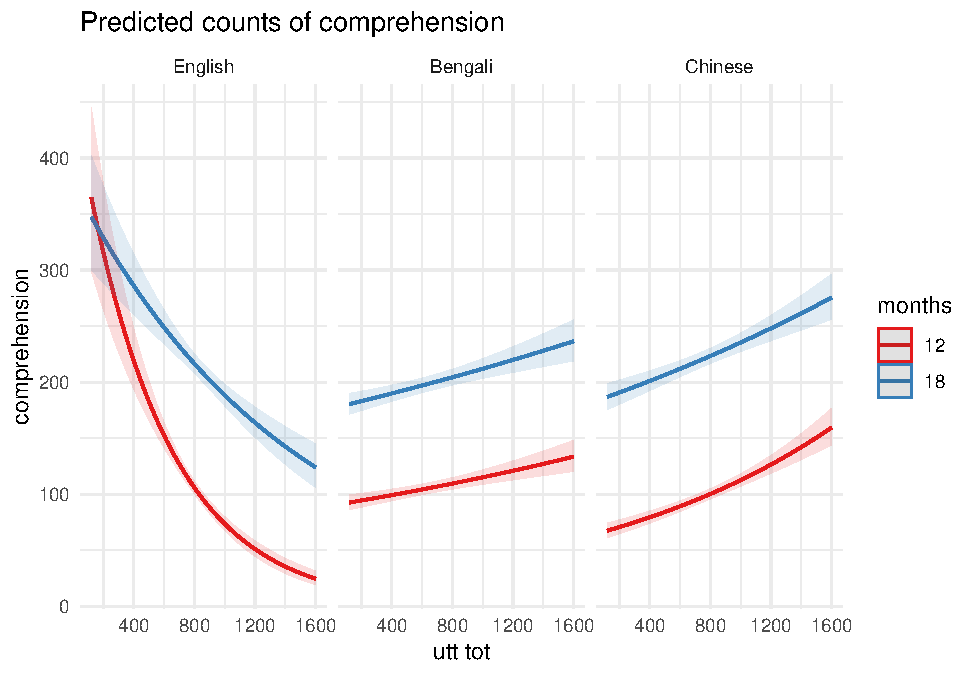
\includegraphics{supplement_files/figure-latex/utt-lm-2-plot-1.pdf}

\hypertarget{contingent-talks}{%
\subsubsection{Contingent talks}\label{contingent-talks}}

\begin{Shaded}
\begin{Highlighting}[]
\NormalTok{ct_lm <-}\StringTok{ }\KeywordTok{glm}\NormalTok{(}
\NormalTok{  comprehension }\OperatorTok{~}
\StringTok{    }\NormalTok{ct_tot }\OperatorTok{*}
\StringTok{    }\NormalTok{months }\OperatorTok{*}
\StringTok{    }\NormalTok{background,}
  \DataTypeTok{data =} \KeywordTok{filter}\NormalTok{(vocab, ct_tot }\OperatorTok{<}\StringTok{ }\DecValTok{30}\NormalTok{)}
\NormalTok{)}
\KeywordTok{summary}\NormalTok{(ct_lm)}
\end{Highlighting}
\end{Shaded}

\begin{verbatim}
## 
## Call:
## glm(formula = comprehension ~ ct_tot * months * background, data = filter(vocab, 
##     ct_tot < 30))
## 
## Deviance Residuals: 
##      Min        1Q    Median        3Q       Max  
## -160.410   -51.991    -3.355    43.823   233.163  
## 
## Coefficients:
##                                   Estimate Std. Error t value Pr(>|t|)    
## (Intercept)                        104.355     25.266   4.130 7.79e-05 ***
## ct_tot                              -1.393      2.720  -0.512  0.60979    
## months18                           106.394     36.217   2.938  0.00415 ** 
## backgroundBengali                  -14.835     33.882  -0.438  0.66249    
## backgroundChinese                  -32.703     38.356  -0.853  0.39601    
## ct_tot:months18                      3.450      3.853   0.895  0.37279    
## ct_tot:backgroundBengali             5.985      4.997   1.198  0.23403    
## ct_tot:backgroundChinese             5.578      3.777   1.477  0.14302    
## months18:backgroundBengali          -6.323     48.280  -0.131  0.89608    
## months18:backgroundChinese           8.490     54.565   0.156  0.87668    
## ct_tot:months18:backgroundBengali   -6.063      7.071  -0.857  0.39337    
## ct_tot:months18:backgroundChinese   -2.572      5.346  -0.481  0.63154    
## ---
## Signif. codes:  0 '***' 0.001 '**' 0.01 '*' 0.05 '.' 0.1 ' ' 1
## 
## (Dispersion parameter for gaussian family taken to be 6241.724)
## 
##     Null deviance: 1002089  on 106  degrees of freedom
## Residual deviance:  592964  on  95  degrees of freedom
##   (1 observation deleted due to missingness)
## AIC: 1252
## 
## Number of Fisher Scoring iterations: 2
\end{verbatim}

\begin{Shaded}
\begin{Highlighting}[]
\KeywordTok{plot_model}\NormalTok{(ct_lm, }\DataTypeTok{type =} \StringTok{"pred"}\NormalTok{, }\DataTypeTok{terms =} \KeywordTok{c}\NormalTok{(}\StringTok{"ct_tot"}\NormalTok{, }\StringTok{"months"}\NormalTok{, }\StringTok{"background"}\NormalTok{))}
\end{Highlighting}
\end{Shaded}

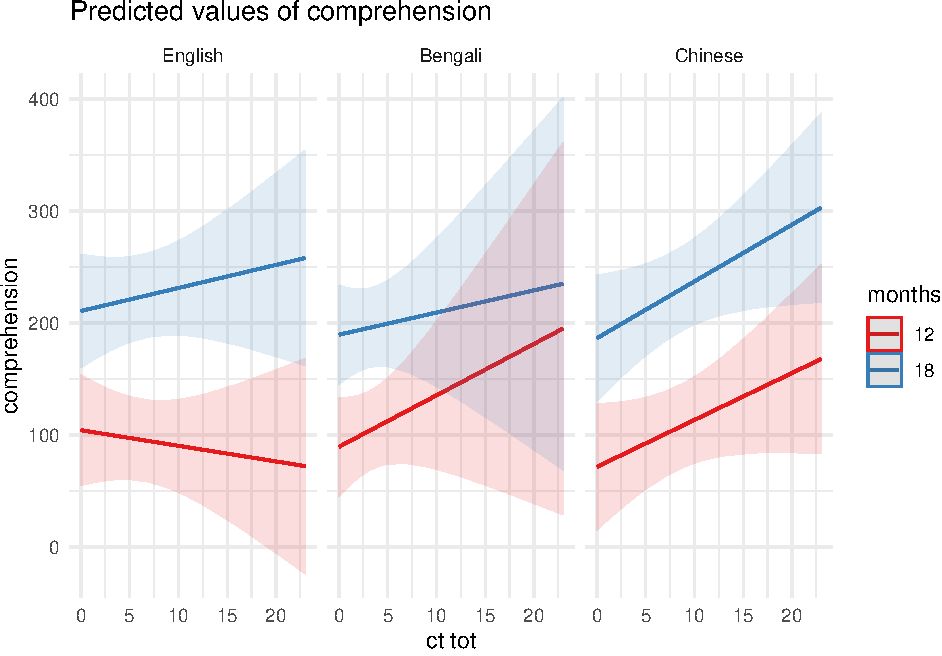
\includegraphics{supplement_files/figure-latex/ct-lm-2-plot-1.pdf}

\hypertarget{production-at-12-and-18-months}{%
\subsection{Production at 12 and 18
months}\label{production-at-12-and-18-months}}

\hypertarget{all-gestures-combined-1}{%
\subsubsection{All gestures combined}\label{all-gestures-combined-1}}

\begin{Shaded}
\begin{Highlighting}[]
\NormalTok{all_gest_prod <-}\StringTok{ }\KeywordTok{glm}\NormalTok{(}
\NormalTok{  production }\OperatorTok{~}
\StringTok{    }\NormalTok{count_tot }\OperatorTok{*}
\StringTok{    }\NormalTok{months }\OperatorTok{*}
\StringTok{    }\NormalTok{background,}
  \DataTypeTok{data =}\NormalTok{ vocab}
\NormalTok{)}
\KeywordTok{summary}\NormalTok{(all_gest_prod)}
\end{Highlighting}
\end{Shaded}

\begin{verbatim}
## 
## Call:
## glm(formula = production ~ count_tot * months * background, data = vocab)
## 
## Deviance Residuals: 
##     Min       1Q   Median       3Q      Max  
## -75.168  -17.714   -3.349    3.721  291.354  
## 
## Coefficients:
##                                        Estimate Std. Error t value Pr(>|t|)   
## (Intercept)                            7.866254  13.736299   0.573   0.5682   
## count_tot                              0.055817   0.281626   0.198   0.8433   
## months18                              20.745124  19.800182   1.048   0.2973   
## backgroundBengali                      1.832536  27.019970   0.068   0.9461   
## backgroundChinese                     -5.841595  23.490202  -0.249   0.8041   
## count_tot:months18                     1.190703   0.400479   2.973   0.0037 **
## count_tot:backgroundBengali           -0.065532   0.595256  -0.110   0.9126   
## count_tot:backgroundChinese           -0.006638   0.479355  -0.014   0.9890   
## months18:backgroundBengali            14.616833  38.403554   0.381   0.7043   
## months18:backgroundChinese           -38.757881  33.440313  -1.159   0.2492   
## count_tot:months18:backgroundBengali  -1.249284   0.842863  -1.482   0.1415   
## count_tot:months18:backgroundChinese   0.396060   0.679205   0.583   0.5611   
## ---
## Signif. codes:  0 '***' 0.001 '**' 0.01 '*' 0.05 '.' 0.1 ' ' 1
## 
## (Dispersion parameter for gaussian family taken to be 2166.208)
## 
##     Null deviance: 359458  on 110  degrees of freedom
## Residual deviance: 214455  on  99  degrees of freedom
##   (9 observations deleted due to missingness)
## AIC: 1180.9
## 
## Number of Fisher Scoring iterations: 2
\end{verbatim}

\begin{Shaded}
\begin{Highlighting}[]
\KeywordTok{plot_model}\NormalTok{(all_gest_prod, }\DataTypeTok{type =} \StringTok{"pred"}\NormalTok{, }\DataTypeTok{terms =} \KeywordTok{c}\NormalTok{(}\StringTok{"count_tot"}\NormalTok{, }\StringTok{"months"}\NormalTok{, }\StringTok{"background"}\NormalTok{))}
\end{Highlighting}
\end{Shaded}

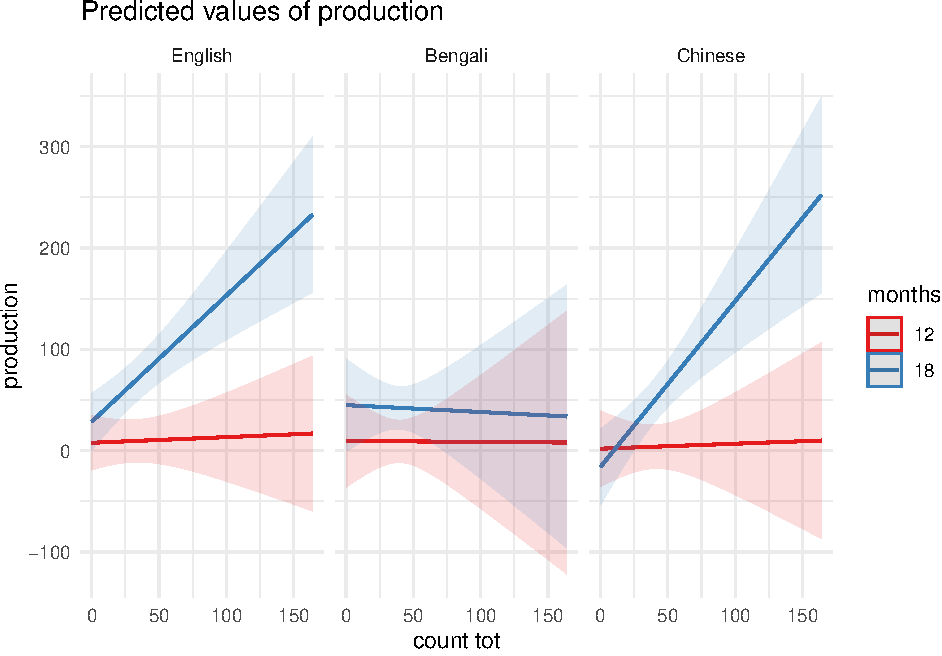
\includegraphics{supplement_files/figure-latex/all-gest-lm-2-undsay-plot-1.pdf}

\hypertarget{hogs-point}{%
\subsubsection{HoGs + point}\label{hogs-point}}

\begin{Shaded}
\begin{Highlighting}[]
\NormalTok{hgp_prod <-}\StringTok{ }\KeywordTok{glm}\NormalTok{(}
\NormalTok{  production }\OperatorTok{~}
\StringTok{    }\NormalTok{hgp_tot }\OperatorTok{*}
\StringTok{    }\NormalTok{months }\OperatorTok{*}
\StringTok{    }\NormalTok{background,}
  \DataTypeTok{data =}\NormalTok{ vocab}
\NormalTok{)}
\KeywordTok{summary}\NormalTok{(hgp_prod)}
\end{Highlighting}
\end{Shaded}

\begin{verbatim}
## 
## Call:
## glm(formula = production ~ hgp_tot * months * background, data = vocab)
## 
## Deviance Residuals: 
##     Min       1Q   Median       3Q      Max  
## -83.961  -17.654   -3.427    3.763  292.162  
## 
## Coefficients:
##                                      Estimate Std. Error t value Pr(>|t|)   
## (Intercept)                          8.792921  12.861066   0.684  0.49577   
## hgp_tot                              0.032679   0.286338   0.114  0.90937   
## months18                            27.819509  18.537964   1.501  0.13662   
## backgroundBengali                    0.760068  24.274303   0.031  0.97508   
## backgroundChinese                   -5.891032  21.174502  -0.278  0.78143   
## hgp_tot:months18                     1.226040   0.407058   3.012  0.00329 **
## hgp_tot:backgroundBengali           -0.041103   0.683926  -0.060  0.95220   
## hgp_tot:backgroundChinese            0.001998   0.489873   0.004  0.99675   
## months18:backgroundBengali          10.491813  34.515585   0.304  0.76179   
## months18:backgroundChinese         -27.089338  30.158931  -0.898  0.37125   
## hgp_tot:months18:backgroundBengali  -1.412798   0.968105  -1.459  0.14764   
## hgp_tot:months18:backgroundChinese   0.194761   0.694023   0.281  0.77958   
## ---
## Signif. codes:  0 '***' 0.001 '**' 0.01 '*' 0.05 '.' 0.1 ' ' 1
## 
## (Dispersion parameter for gaussian family taken to be 2241.502)
## 
##     Null deviance: 359458  on 110  degrees of freedom
## Residual deviance: 221909  on  99  degrees of freedom
##   (9 observations deleted due to missingness)
## AIC: 1184.7
## 
## Number of Fisher Scoring iterations: 2
\end{verbatim}

\begin{Shaded}
\begin{Highlighting}[]
\KeywordTok{plot_model}\NormalTok{(hgp_prod, }\DataTypeTok{type =} \StringTok{"pred"}\NormalTok{, }\DataTypeTok{terms =} \KeywordTok{c}\NormalTok{(}\StringTok{"hgp_tot"}\NormalTok{, }\StringTok{"months"}\NormalTok{, }\StringTok{"background"}\NormalTok{))}
\end{Highlighting}
\end{Shaded}

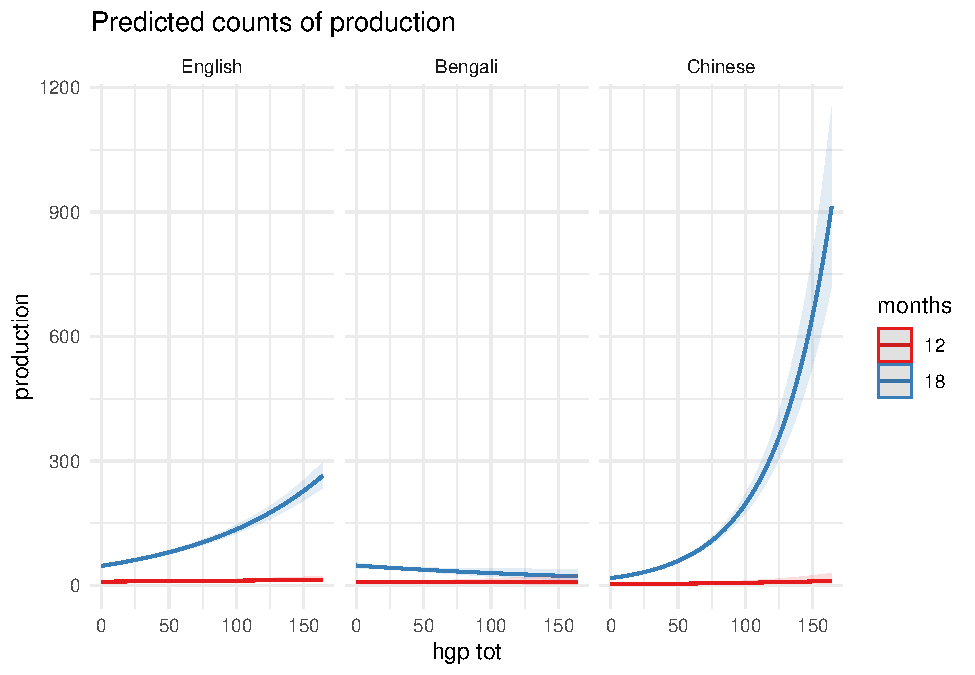
\includegraphics{supplement_files/figure-latex/hgp-lm-2-undsay-plot-1.pdf}

\hypertarget{reaches-2}{%
\subsubsection{Reaches}\label{reaches-2}}

\begin{Shaded}
\begin{Highlighting}[]
\NormalTok{reach_prod <-}\StringTok{ }\KeywordTok{glm}\NormalTok{(}
\NormalTok{  production }\OperatorTok{~}
\StringTok{    }\NormalTok{reach_tot }\OperatorTok{*}
\StringTok{    }\NormalTok{months }\OperatorTok{*}
\StringTok{    }\NormalTok{background,}
  \DataTypeTok{data =}\NormalTok{ vocab}
\NormalTok{)}
\KeywordTok{summary}\NormalTok{(reach_prod)}
\end{Highlighting}
\end{Shaded}

\begin{verbatim}
## 
## Call:
## glm(formula = production ~ reach_tot * months * background, data = vocab)
## 
## Deviance Residuals: 
##     Min       1Q   Median       3Q      Max  
## -75.884  -23.583   -3.345    4.233  288.621  
## 
## Coefficients:
##                                      Estimate Std. Error t value Pr(>|t|)   
## (Intercept)                            4.5636    17.2142   0.265   0.7915   
## reach_tot                              0.7563     1.8361   0.412   0.6813   
## months18                              67.1258    24.5465   2.735   0.0074 **
## backgroundBengali                      5.1348    29.7331   0.173   0.8632   
## backgroundChinese                     -3.8276    28.5298  -0.134   0.8935   
## reach_tot:months18                    -1.2347     2.5970  -0.475   0.6355   
## reach_tot:backgroundBengali           -0.7903     2.6148  -0.302   0.7631   
## reach_tot:backgroundChinese           -0.3723     2.8935  -0.129   0.8979   
## months18:backgroundBengali           -42.7283    42.1663  -1.013   0.3134   
## months18:backgroundChinese           -61.9845    40.4694  -1.532   0.1288   
## reach_tot:months18:backgroundBengali   2.0031     3.6981   0.542   0.5893   
## reach_tot:months18:backgroundChinese   6.0089     4.0923   1.468   0.1452   
## ---
## Signif. codes:  0 '***' 0.001 '**' 0.01 '*' 0.05 '.' 0.1 ' ' 1
## 
## (Dispersion parameter for gaussian family taken to be 2813.16)
## 
##     Null deviance: 359458  on 110  degrees of freedom
## Residual deviance: 278503  on  99  degrees of freedom
##   (9 observations deleted due to missingness)
## AIC: 1209.9
## 
## Number of Fisher Scoring iterations: 2
\end{verbatim}

\begin{Shaded}
\begin{Highlighting}[]
\KeywordTok{plot_model}\NormalTok{(reach_prod, }\DataTypeTok{type =} \StringTok{"pred"}\NormalTok{, }\DataTypeTok{terms =} \KeywordTok{c}\NormalTok{(}\StringTok{"reach_tot"}\NormalTok{, }\StringTok{"months"}\NormalTok{, }\StringTok{"background"}\NormalTok{))}
\end{Highlighting}
\end{Shaded}

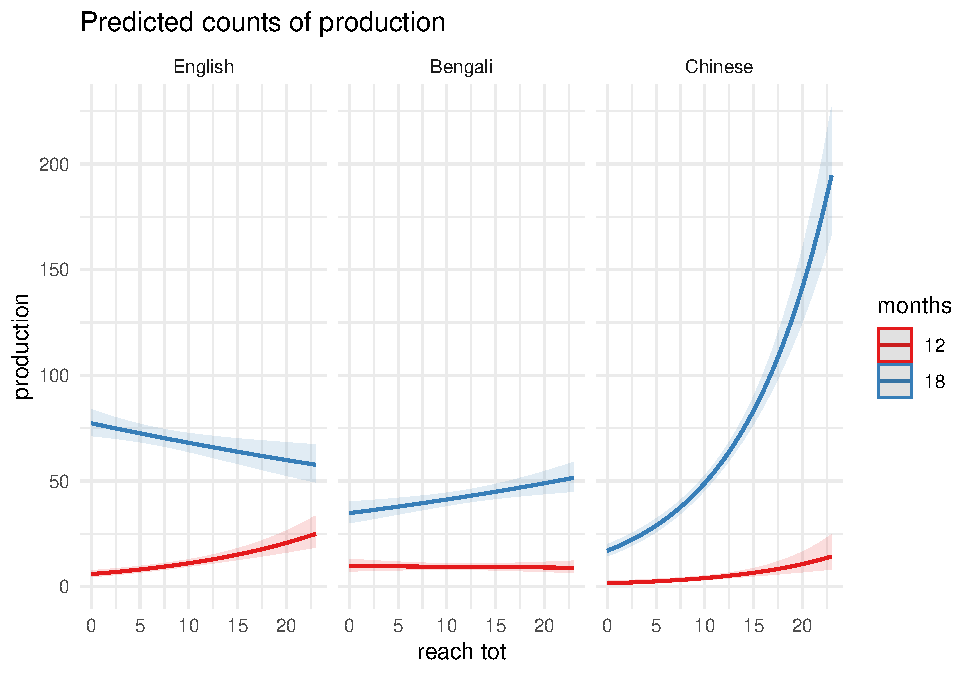
\includegraphics{supplement_files/figure-latex/reach-lm-2-undsay-plot-1.pdf}

\hypertarget{maternal-utterances-1}{%
\subsubsection{Maternal utterances}\label{maternal-utterances-1}}

\begin{Shaded}
\begin{Highlighting}[]
\NormalTok{utt_prod <-}\StringTok{ }\KeywordTok{glm}\NormalTok{(}
\NormalTok{  production }\OperatorTok{~}
\StringTok{    }\NormalTok{utt_tot }\OperatorTok{*}
\StringTok{    }\NormalTok{months }\OperatorTok{*}
\StringTok{    }\NormalTok{background,}
  \DataTypeTok{data =}\NormalTok{ vocab}
\NormalTok{)}
\KeywordTok{summary}\NormalTok{(utt_prod)}
\end{Highlighting}
\end{Shaded}

\begin{verbatim}
## 
## Call:
## glm(formula = production ~ utt_tot * months * background, data = vocab)
## 
## Deviance Residuals: 
##      Min        1Q    Median        3Q       Max  
## -116.668   -17.309    -3.129     3.772   215.516  
## 
## Coefficients:
##                                      Estimate Std. Error t value Pr(>|t|)
## (Intercept)                          1.326517  41.130133   0.032    0.974
## utt_tot                              0.005932   0.048877   0.121    0.904
## months18                            26.710518  58.994380   0.453    0.652
## backgroundBengali                    2.338218  45.617854   0.051    0.959
## backgroundChinese                    1.127511  48.233863   0.023    0.981
## utt_tot:months18                     0.017534   0.069563   0.252    0.802
## utt_tot:backgroundBengali            0.002871   0.055449   0.052    0.959
## utt_tot:backgroundChinese           -0.004009   0.057492  -0.070    0.945
## months18:backgroundBengali         -36.716096  65.260543  -0.563    0.575
## months18:backgroundChinese          12.482321  68.920043   0.181    0.857
## utt_tot:months18:backgroundBengali   0.057540   0.078806   0.730    0.467
## utt_tot:months18:backgroundChinese  -0.012033   0.081681  -0.147    0.883
## 
## (Dispersion parameter for gaussian family taken to be 2282.756)
## 
##     Null deviance: 268717  on 100  degrees of freedom
## Residual deviance: 203165  on  89  degrees of freedom
##   (19 observations deleted due to missingness)
## AIC: 1080.9
## 
## Number of Fisher Scoring iterations: 2
\end{verbatim}

\begin{Shaded}
\begin{Highlighting}[]
\KeywordTok{plot_model}\NormalTok{(utt_prod, }\DataTypeTok{type =} \StringTok{"pred"}\NormalTok{, }\DataTypeTok{terms =} \KeywordTok{c}\NormalTok{(}\StringTok{"utt_tot"}\NormalTok{, }\StringTok{"months"}\NormalTok{, }\StringTok{"background"}\NormalTok{))}
\end{Highlighting}
\end{Shaded}

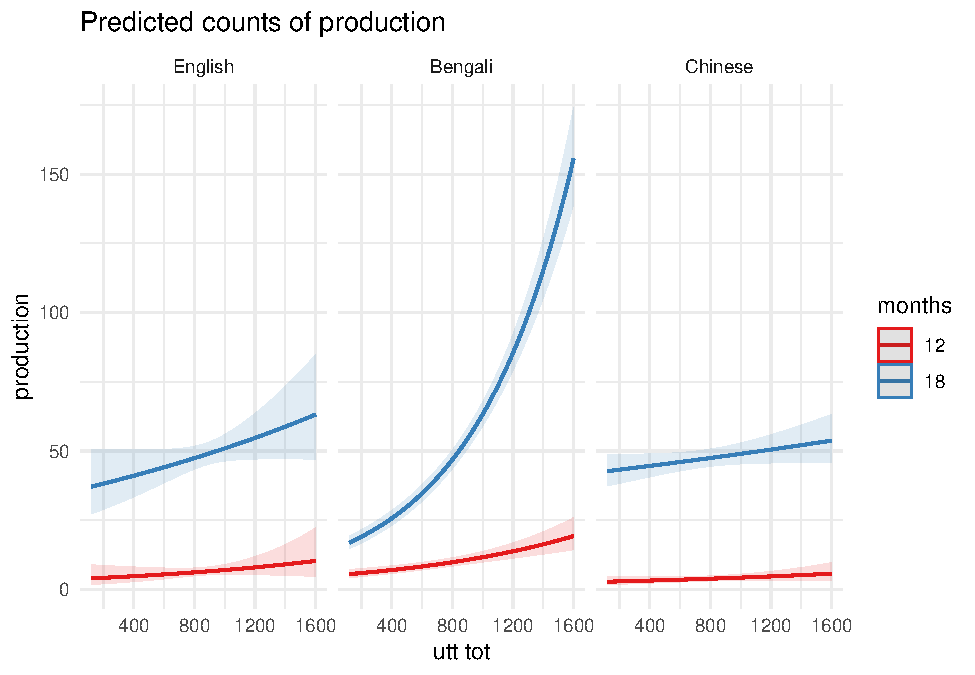
\includegraphics{supplement_files/figure-latex/utt-lm-2-undsay-plot-1.pdf}

\hypertarget{contingent-talks-1}{%
\subsubsection{Contingent talks}\label{contingent-talks-1}}

\begin{Shaded}
\begin{Highlighting}[]
\NormalTok{ct_prod <-}\StringTok{ }\KeywordTok{glm}\NormalTok{(}
\NormalTok{  production }\OperatorTok{~}
\StringTok{    }\NormalTok{ct_tot }\OperatorTok{*}
\StringTok{    }\NormalTok{months }\OperatorTok{*}
\StringTok{    }\NormalTok{background,}
  \DataTypeTok{data =} \KeywordTok{filter}\NormalTok{(vocab, ct_tot }\OperatorTok{<}\StringTok{ }\DecValTok{30}\NormalTok{)}
\NormalTok{)}
\KeywordTok{summary}\NormalTok{(ct_prod)}
\end{Highlighting}
\end{Shaded}

\begin{verbatim}
## 
## Call:
## glm(formula = production ~ ct_tot * months * background, data = filter(vocab, 
##     ct_tot < 30))
## 
## Deviance Residuals: 
##      Min        1Q    Median        3Q       Max  
## -109.012   -15.470    -2.756     4.862   197.095  
## 
## Coefficients:
##                                   Estimate Std. Error t value Pr(>|t|)  
## (Intercept)                         6.0079    14.3315   0.419   0.6760  
## ct_tot                              0.5828     1.5429   0.378   0.7065  
## months18                           19.0797    20.5435   0.929   0.3554  
## backgroundBengali                  -0.5135    19.2192  -0.027   0.9787  
## backgroundChinese                  -4.7043    21.7567  -0.216   0.8293  
## ct_tot:months18                     4.8989     2.1856   2.241   0.0273 *
## ct_tot:backgroundBengali            0.6075     2.8347   0.214   0.8308  
## ct_tot:backgroundChinese           -0.2911     2.1424  -0.136   0.8922  
## months18:backgroundBengali        -18.4869    27.3863  -0.675   0.5013  
## months18:backgroundChinese          8.1442    30.9510   0.263   0.7930  
## ct_tot:months18:backgroundBengali   5.7033     4.0108   1.422   0.1583  
## ct_tot:months18:backgroundChinese  -2.4976     3.0324  -0.824   0.4122  
## ---
## Signif. codes:  0 '***' 0.001 '**' 0.01 '*' 0.05 '.' 0.1 ' ' 1
## 
## (Dispersion parameter for gaussian family taken to be 2008.297)
## 
##     Null deviance: 326620  on 106  degrees of freedom
## Residual deviance: 190788  on  95  degrees of freedom
##   (1 observation deleted due to missingness)
## AIC: 1130.7
## 
## Number of Fisher Scoring iterations: 2
\end{verbatim}

\begin{Shaded}
\begin{Highlighting}[]
\KeywordTok{plot_model}\NormalTok{(ct_prod, }\DataTypeTok{type =} \StringTok{"pred"}\NormalTok{, }\DataTypeTok{terms =} \KeywordTok{c}\NormalTok{(}\StringTok{"ct_tot"}\NormalTok{, }\StringTok{"months"}\NormalTok{, }\StringTok{"background"}\NormalTok{))}
\end{Highlighting}
\end{Shaded}

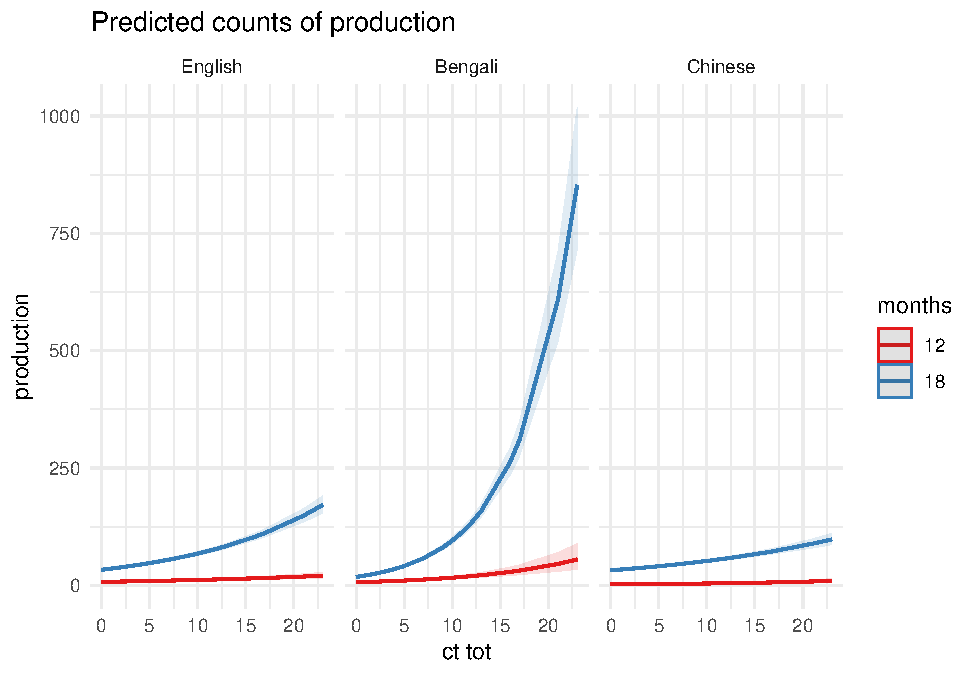
\includegraphics{supplement_files/figure-latex/ct-lm-2-undsay-plot-1.pdf}

\newpage

\hypertarget{number-of-observations}{%
\section{Number of observations}\label{number-of-observations}}

The following sections report the number of observations (excluding NAs)
used in the models above.

\hypertarget{analysis-1a}{%
\subsection{Analysis 1a}\label{analysis-1a}}

\hypertarget{reaches-3}{%
\subsubsection{Reaches}\label{reaches-3}}

\begin{Shaded}
\begin{Highlighting}[]
\NormalTok{reach_tot }\OperatorTok
\StringTok{  }\KeywordTok{group_by}\NormalTok{(back_o, months) }\OperatorTok
\StringTok{  }\KeywordTok{na.omit}\NormalTok{() }\OperatorTok
\StringTok{  }\KeywordTok{summarise}\NormalTok{(}\DataTypeTok{n =} \KeywordTok{n}\NormalTok{())}
\end{Highlighting}
\end{Shaded}

\begin{verbatim}
## # A tibble: 9 x 3
## # Groups:   back_o [3]
##   back_o  months     n
##   <ord>    <dbl> <int>
## 1 English     10    20
## 2 English     11    20
## 3 English     12    19
## 4 Bengali     10    20
## 5 Bengali     11    19
## 6 Bengali     12    19
## 7 Chinese     10    18
## 8 Chinese     11    19
## 9 Chinese     12    20
\end{verbatim}

\hypertarget{hogs-1}{%
\subsubsection{HoGs}\label{hogs-1}}

\begin{Shaded}
\begin{Highlighting}[]
\NormalTok{hg_tot }\OperatorTok
\StringTok{  }\KeywordTok{group_by}\NormalTok{(back_o, months) }\OperatorTok
\StringTok{  }\KeywordTok{na.omit}\NormalTok{() }\OperatorTok
\StringTok{  }\KeywordTok{summarise}\NormalTok{(}\DataTypeTok{n =} \KeywordTok{n}\NormalTok{())}
\end{Highlighting}
\end{Shaded}

\begin{verbatim}
## # A tibble: 9 x 3
## # Groups:   back_o [3]
##   back_o  months     n
##   <ord>    <dbl> <int>
## 1 English     10    20
## 2 English     11    20
## 3 English     12    19
## 4 Bengali     10    20
## 5 Bengali     11    19
## 6 Bengali     12    19
## 7 Chinese     10    18
## 8 Chinese     11    19
## 9 Chinese     12    20
\end{verbatim}

\hypertarget{points}{%
\subsubsection{Points}\label{points}}

\begin{Shaded}
\begin{Highlighting}[]
\NormalTok{point_tot }\OperatorTok
\StringTok{  }\KeywordTok{group_by}\NormalTok{(back_o, months) }\OperatorTok
\StringTok{  }\KeywordTok{na.omit}\NormalTok{() }\OperatorTok
\StringTok{  }\KeywordTok{summarise}\NormalTok{(}\DataTypeTok{n =} \KeywordTok{n}\NormalTok{())}
\end{Highlighting}
\end{Shaded}

\begin{verbatim}
## # A tibble: 9 x 3
## # Groups:   back_o [3]
##   back_o  months     n
##   <ord>    <dbl> <int>
## 1 English     10    20
## 2 English     11    20
## 3 English     12    19
## 4 Bengali     10    20
## 5 Bengali     11    19
## 6 Bengali     12    19
## 7 Chinese     10    18
## 8 Chinese     11    19
## 9 Chinese     12    20
\end{verbatim}

\hypertarget{analysis-1b}{%
\subsection{Analysis 1b}\label{analysis-1b}}

\hypertarget{maternal-utterances-2}{%
\subsubsection{Maternal utterances}\label{maternal-utterances-2}}

\begin{Shaded}
\begin{Highlighting}[]
\NormalTok{utterances_tot }\OperatorTok
\StringTok{  }\KeywordTok{group_by}\NormalTok{(back_o, months) }\OperatorTok
\StringTok{  }\KeywordTok{na.omit}\NormalTok{() }\OperatorTok
\StringTok{  }\KeywordTok{summarise}\NormalTok{(}\DataTypeTok{n =} \KeywordTok{n}\NormalTok{())}
\end{Highlighting}
\end{Shaded}

\begin{verbatim}
## # A tibble: 9 x 3
## # Groups:   back_o [3]
##   back_o  months     n
##   <ord>    <dbl> <int>
## 1 English     10    18
## 2 English     11    19
## 3 English     12    17
## 4 Bengali     10    20
## 5 Bengali     11    19
## 6 Bengali     12    18
## 7 Chinese     10    19
## 8 Chinese     11    20
## 9 Chinese     12    20
\end{verbatim}

\hypertarget{maternal-cts}{%
\subsubsection{Maternal CTs}\label{maternal-cts}}

\begin{Shaded}
\begin{Highlighting}[]
\NormalTok{all_tot }\OperatorTok
\StringTok{  }\KeywordTok{group_by}\NormalTok{(back_o, months) }\OperatorTok
\StringTok{  }\KeywordTok{na.omit}\NormalTok{() }\OperatorTok
\StringTok{  }\KeywordTok{summarise}\NormalTok{(}\DataTypeTok{n =} \KeywordTok{n}\NormalTok{())}
\end{Highlighting}
\end{Shaded}

\begin{verbatim}
## # A tibble: 9 x 3
## # Groups:   back_o [3]
##   back_o  months     n
##   <ord>    <dbl> <int>
## 1 English     10    20
## 2 English     11    20
## 3 English     12    19
## 4 Bengali     10    20
## 5 Bengali     11    19
## 6 Bengali     12    19
## 7 Chinese     10    18
## 8 Chinese     11    19
## 9 Chinese     12    20
\end{verbatim}

\hypertarget{analysis-1c}{%
\subsection{Analysis 1c}\label{analysis-1c}}

\hypertarget{reaches-4}{%
\subsubsection{Reaches}\label{reaches-4}}

\begin{Shaded}
\begin{Highlighting}[]
\NormalTok{reach_point_lead }\OperatorTok
\StringTok{  }\KeywordTok{group_by}\NormalTok{(back_o) }\OperatorTok
\StringTok{  }\KeywordTok{na.omit}\NormalTok{() }\OperatorTok
\StringTok{  }\KeywordTok{summarise}\NormalTok{(}\DataTypeTok{n =} \KeywordTok{n}\NormalTok{())}
\end{Highlighting}
\end{Shaded}

\begin{verbatim}
## # A tibble: 3 x 2
##   back_o      n
##   <ord>   <int>
## 1 English    39
## 2 Bengali    38
## 3 Chinese    37
\end{verbatim}

\hypertarget{hogs-2}{%
\subsubsection{HoGs}\label{hogs-2}}

\begin{Shaded}
\begin{Highlighting}[]
\NormalTok{hg_point_lead }\OperatorTok
\StringTok{  }\KeywordTok{group_by}\NormalTok{(back_o) }\OperatorTok
\StringTok{  }\KeywordTok{na.omit}\NormalTok{() }\OperatorTok
\StringTok{  }\KeywordTok{summarise}\NormalTok{(}\DataTypeTok{n =} \KeywordTok{n}\NormalTok{())}
\end{Highlighting}
\end{Shaded}

\begin{verbatim}
## # A tibble: 3 x 2
##   back_o      n
##   <ord>   <int>
## 1 English    39
## 2 Bengali    38
## 3 Chinese    37
\end{verbatim}

\hypertarget{analysis-2}{%
\subsection{Analysis 2}\label{analysis-2}}

The counts apply both to the comprehension and production analyses.

\begin{Shaded}
\begin{Highlighting}[]
\NormalTok{vocab }\OperatorTok
\StringTok{  }\KeywordTok{group_by}\NormalTok{(background) }\OperatorTok
\StringTok{  }\KeywordTok{na.omit}\NormalTok{() }\OperatorTok
\StringTok{  }\KeywordTok{summarise}\NormalTok{(}\DataTypeTok{n =} \KeywordTok{n}\NormalTok{())}
\end{Highlighting}
\end{Shaded}

\begin{verbatim}
## # A tibble: 3 x 2
##   background     n
##   <fct>      <int>
## 1 English       27
## 2 Bengali       34
## 3 Chinese       34
\end{verbatim}

\hypertarget{correlation-of-vocabulary-scores-and-maternal-scores}{%
\section{Correlation of vocabulary scores and maternal
scores}\label{correlation-of-vocabulary-scores-and-maternal-scores}}

\begin{Shaded}
\begin{Highlighting}[]
\NormalTok{vocab }\OperatorTok
\StringTok{  }\KeywordTok{ggplot}\NormalTok{(}\KeywordTok{aes}\NormalTok{(comprehension, production)) }\OperatorTok{+}
\StringTok{  }\KeywordTok{geom_point}\NormalTok{() }\OperatorTok{+}
\StringTok{  }\KeywordTok{geom_smooth}\NormalTok{(}\DataTypeTok{method =} \StringTok{"glm"}\NormalTok{, }\DataTypeTok{method.args =} \KeywordTok{list}\NormalTok{(}\DataTypeTok{family =}\NormalTok{ poisson))}
\end{Highlighting}
\end{Shaded}

\begin{verbatim}
## Warning: Removed 3 rows containing non-finite values (stat_smooth).
\end{verbatim}

\begin{verbatim}
## Warning: Removed 3 rows containing missing values (geom_point).
\end{verbatim}

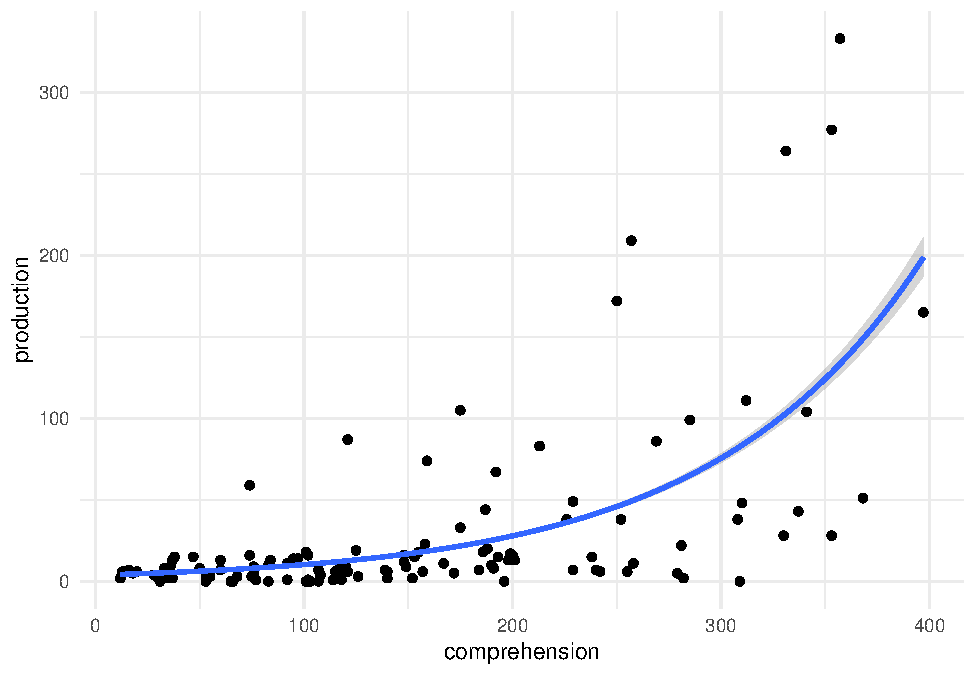
\includegraphics{supplement_files/figure-latex/vocab-cor-1.pdf}

\begin{Shaded}
\begin{Highlighting}[]
\NormalTok{all_tot }\OperatorTok
\StringTok{  }\KeywordTok{left_join}\NormalTok{(utterances_tot) }\OperatorTok
\StringTok{  }\KeywordTok{ggplot}\NormalTok{(}\KeywordTok{aes}\NormalTok{(utterances, ct)) }\OperatorTok{+}
\StringTok{  }\KeywordTok{geom_point}\NormalTok{() }\OperatorTok{+}
\StringTok{  }\KeywordTok{geom_smooth}\NormalTok{(}\DataTypeTok{method =} \StringTok{"glm"}\NormalTok{, }\DataTypeTok{method.args =} \KeywordTok{list}\NormalTok{(}\DataTypeTok{family =}\NormalTok{ poisson))}
\end{Highlighting}
\end{Shaded}

\begin{verbatim}
## Joining, by = c("dyad", "back_o", "months")
\end{verbatim}

\begin{verbatim}
## Warning: Removed 12 rows containing non-finite values (stat_smooth).
\end{verbatim}

\begin{verbatim}
## Warning: Removed 12 rows containing missing values (geom_point).
\end{verbatim}

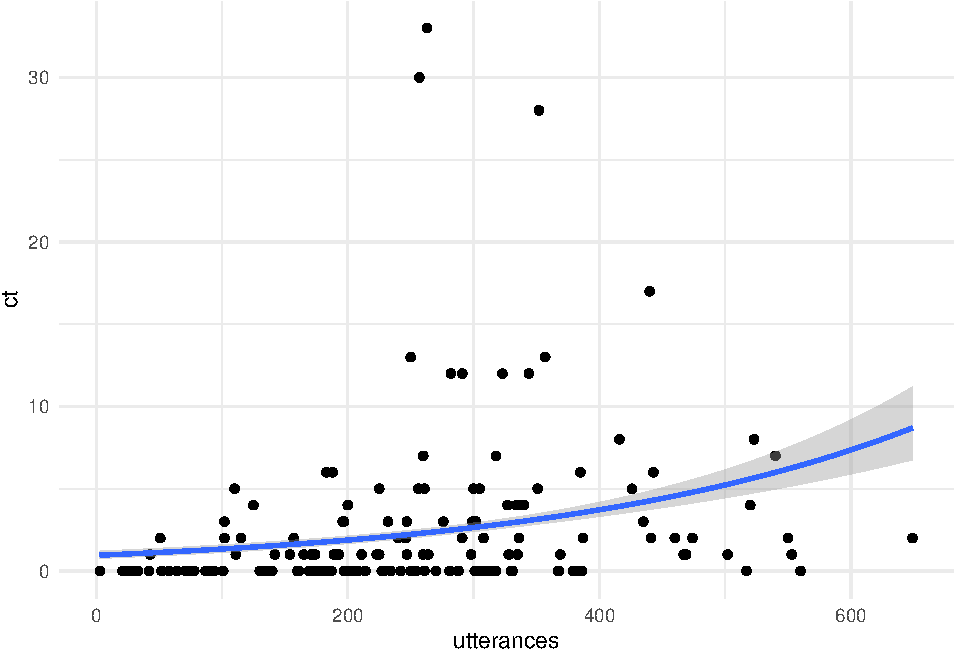
\includegraphics{supplement_files/figure-latex/maternal-cor-1.pdf}

\hypertarget{r-session}{%
\section{R session}\label{r-session}}

\begin{Shaded}
\begin{Highlighting}[]
\KeywordTok{sessionInfo}\NormalTok{()}
\end{Highlighting}
\end{Shaded}

\begin{verbatim}
## R version 3.5.3 (2019-03-11)
## Platform: x86_64-apple-darwin15.6.0 (64-bit)
## Running under: macOS  10.15.2
## 
## Matrix products: default
## BLAS: /Library/Frameworks/R.framework/Versions/3.5/Resources/lib/libRblas.0.dylib
## LAPACK: /Library/Frameworks/R.framework/Versions/3.5/Resources/lib/libRlapack.dylib
## 
## locale:
## [1] en_GB.UTF-8/en_GB.UTF-8/en_GB.UTF-8/C/en_GB.UTF-8/en_GB.UTF-8
## 
## attached base packages:
## [1] stats     graphics  grDevices utils     datasets  methods   base     
## 
## other attached packages:
##  [1] sjPlot_2.8.1      simr_1.0.5        effects_4.1-4     carData_3.0-3    
##  [5] lmerTest_3.1-0    lme4_1.1-21       Matrix_1.2-18     tidymv_2.2.0     
##  [9] itsadug_2.3       plotfunctions_1.3 mgcv_1.8-31       nlme_3.1-142     
## [13] forcats_0.4.0     stringr_1.4.0     dplyr_0.8.3       purrr_0.3.3      
## [17] readr_1.3.1       tidyr_1.0.0       tibble_2.1.3      ggplot2_3.2.1    
## [21] tidyverse_1.3.0   MASS_7.3-51.4    
## 
## loaded via a namespace (and not attached):
##   [1] TH.data_1.0-10      minqa_1.2.4         colorspace_1.4-1   
##   [4] rio_0.5.16          sjlabelled_1.1.1    snakecase_0.11.0   
##   [7] estimability_1.3    parameters_0.3.0    fs_1.3.1           
##  [10] rstudioapi_0.10     farver_2.0.1        ggrepel_0.8.1      
##  [13] mvtnorm_1.0-11      fansi_0.4.0         lubridate_1.7.4    
##  [16] xml2_1.2.2          codetools_0.2-16    splines_3.5.3      
##  [19] mnormt_1.5-5        knitr_1.26          sjmisc_2.8.2       
##  [22] zeallot_0.1.0       jsonlite_1.6        nloptr_1.2.1       
##  [25] ggeffects_0.13.0    pbkrtest_0.4-7      broom_0.5.2        
##  [28] binom_1.1-1         dbplyr_1.4.2        effectsize_0.0.1   
##  [31] compiler_3.5.3      httr_1.4.1          sjstats_0.17.7     
##  [34] emmeans_1.4.3.01    backports_1.1.5     assertthat_0.2.1   
##  [37] lazyeval_0.2.2      survey_3.36         cli_2.0.0          
##  [40] htmltools_0.4.0     tools_3.5.3         coda_0.19-3        
##  [43] gtable_0.3.0        glue_1.3.1          Rcpp_1.0.3         
##  [46] cellranger_1.1.0    vctrs_0.2.0         iterators_1.0.12   
##  [49] psych_1.8.12        insight_0.7.1       xfun_0.11          
##  [52] openxlsx_4.1.4      rvest_0.3.5         lifecycle_0.1.0    
##  [55] zoo_1.8-6           scales_1.1.0        hms_0.5.2          
##  [58] sandwich_2.5-1      parallel_3.5.3      RColorBrewer_1.1-2 
##  [61] yaml_2.2.0          curl_4.3            stringi_1.4.3      
##  [64] bayestestR_0.4.0    plotrix_3.7-7       boot_1.3-23        
##  [67] zip_2.0.4           rlang_0.4.2         pkgconfig_2.0.3    
##  [70] evaluate_0.14       lattice_0.20-38     labeling_0.3       
##  [73] tidyselect_0.2.5    plyr_1.8.4          magrittr_1.5       
##  [76] R6_2.4.1            generics_0.0.2      multcomp_1.4-11    
##  [79] RLRsim_3.1-3        DBI_1.0.0           pillar_1.4.2       
##  [82] haven_2.2.0         foreign_0.8-72      withr_2.1.2        
##  [85] survival_3.1-8      abind_1.4-5         nnet_7.3-12        
##  [88] performance_0.4.0   modelr_0.1.5        crayon_1.3.4       
##  [91] car_3.0-5           utf8_1.1.4          rmarkdown_1.18     
##  [94] grid_3.5.3          readxl_1.3.1        data.table_1.12.6  
##  [97] reprex_0.3.0        digest_0.6.23       xtable_1.8-4       
## [100] numDeriv_2016.8-1.1 munsell_0.5.0       mitools_2.4
\end{verbatim}

\end{document}
